%! TeX program = lualatex
%---------------------------ALLGEMEINE IMPORTS-------------------------------------
\documentclass[12pt,english,ngerman]{scrartcl}
\input{protokoll_template/template.latex/input/shared_preamble.tex}

% Kopfzeile
\ihead{SS22\\
	17.05.2023}

\chead{\textsc{Stark} Matthias --- 12004907 \\
	\textsc{Philipp} Maximilian --- 11839611}

\ohead{FLAB 2 \\
	Interferenz \\ und Polarisation}

% Fußzeile
%todo 
\addbibresource{Interfero.bib}

\usepackage{luacode}

\DeclareSIUnit\px{px}
\DeclareSIUnit\strich{|||}
\DeclareSIUnit\Var{var}
\DeclareSIUnit\VA{VA}
\DeclareSIUnit\bar{bar}

\usepackage{cleveref}

\crefname{enumerate}{Aufzählung}{Aufzählungen}

\begin{document}

\begin{luacode*}
dofile("createExtraPDF.lua")
\end{luacode*}

%
\includepdf{./deckblatt.pdf}
\tableofcontents

\newpage

\section{Aufgabenstellung}\label{Auf}

\subsection{Young'scher Doppelspalt, Beugungsgitter}

\begin{itemize}
	\item Bestimmen Sie das Beugungsmuster von vier Doppelspalten mit (bekannten)
	      unterschiedlichen Spaltbreiten und Spaltabständen. Berechnen Sie aus den
	      Messwerten die Wellenlänge des LASERs.
	\item Erklären Sie die Details der beobachteten Beugungsmuster durch Vergleich mit
	      den berechneten Mustern.
	\item Bestimmen Sie das Beugungsmuster eines Liniengitters und vergleichen Sie mit
	      berechneten Werten. Berechnen Sie aus den Messwerten die Gitterkonstante.
\end{itemize}

\subsection{Polarisation}

\begin{itemize}
	\item Verifizieren Sie das Gesetz von Malus.
	\item Untersuchen Sie den Einfluss des Durchlasswinkels eines weiteren Polarisators
	      zwischen zwei gekreuzten Polarisatoren.
\end{itemize}

\subsection{Michelson Interferometer}

\begin{itemize}
	\item Justieren Sie das Interferometer und generieren Sie ein konzentrisches
	      Interferenzmuster. Bestimmen Sie durch Weglängenänderung die Wellenlänge des
	      LASERs. Wiederholen Sie dies für ein paralleles Interferenzmuster.
	\item Untersuchen Sie den absoluten Weglängenunterschied in den beiden
	      Interferometerarmen, sowie Auflösung und Stabilität des Interferometers.
	\item Untersuchen Sie die Rolle der Polarisation auf die Interferenzfähigkeit des
	      Laserlichts.
\end{itemize}

\newpage

\section{Grundlagen}\label{sec:Grund}

\subsection{Kohärenz}

Die zeitliche Kohärenz bezieht sich auf den Grad der Ähnlichkeit zwischen zwei
Lichtwellen, die von derselben Quelle, aber zu unterschiedlichen Zeiten
ausgesendet werden. Lichtwellen bestehen aus oszillierenden elektrischen und
magnetischen Feldern. Damit es zu eine Interferenz kommt, müssen die beiden
Wellen eine konstante Phasenbeziehung haben. Das bedeutet, dass die
Phasendifferenz zwischen den beiden Wellen über einen längeren Zeitraum
konstant bleiben muss. Ändert sich die Phasenbeziehung schnell, wird von einer
geringen zeitlichen Kohärenz der Wellen ausgegangen. Bleibt die Phasenbeziehung
dagegen über einen langen Zeitraum konstant, so wird von einer hohen zeitlichen
Kohärenz ausgegangen.

Die räumliche Kohärenz hingegen bezieht sich auf den Grad der Ähnlichkeit
zwischen zwei Lichtwellen, die von derselben Quelle, aber an unterschiedlichen
Orten im Raum ausgesendet werden. Damit es zu einer Interferenz kommt, müssen
die beiden Wellen über ihre gesamte Wellenfront eine konstante Phasenbeziehung
aufweisen. Das bedeutet, dass die Phasendifferenz zwischen zwei beliebigen
Punkten der Wellenfronten konstant bleiben sollte. Wenn sich die
Phasenbeziehung über die Wellenfronten hinweg schnell ändert, wird von einer
geringen räumlichen Kohärenz der Wellen ausgegangen. Bleibt die Phasenbeziehung
dagegen über die Wellenfronten hinweg konstant, so wird von einer hohen
räumlichen Kohärenz ausgegangen.

Die Kohärenzlänge ist ein Maß dafür, wie weit sich das Licht unter Beibehaltung
seiner Kohärenz ausbreiten kann. Sie ist die Strecke, über die die
Phasenbeziehung zwischen zwei Punkten auf einer Wellenfront konstant bleibt.
Die Kohärenzlänge verhält sich umgekehrt proportional zur spektralen Bandbreite
der Lichtquelle. Eine schmalbandige Lichtquelle mit einer kleinen spektralen
Bandbreite hat eine große Kohärenzlänge, während eine breitbandige Lichtquelle
mit einer großen spektralen Bandbreite eine kleine Kohärenzlänge hat.

Zur Erzeugung von Interferenzmustern mit Licht ist eine Lichtquelle mit hoher
zeitlicher Kohärenz, hoher räumlicher Kohärenz und einer ausreichend langen
Kohärenzlänge erforderlich. Eine hohe zeitliche Kohärenz gewährleistet, dass
die Phasenbeziehung zwischen zwei Wellen über einen längeren Zeitraum konstant
bleibt, so dass sie konstruktiv oder destruktiv interferieren können. Eine hohe
räumliche Kohärenz stellt sicher, dass die Phasenbeziehung zwischen
verschiedenen Punkten auf den Wellenfronten konstant bleibt, so dass die Wellen
gleichmäßig über das Muster interferieren können. Die Kohärenzlänge bestimmt
die Größe des Bereichs, in dem Interferenz auftreten kann. Eine große
Kohärenzlänge ist notwendig, um gut definierte Interferenzstreifen zu
beobachten, während eine kurze Kohärenzlänge zu verschwommenen oder
verwaschenen Mustern führt.

\subsection{Doppelspalt}

Das Youngsche Doppelspaltexperiment ist ein klassisches Experiment, das die
Wellennatur des Lichts und das Phänomen der Interferenz demonstriert. Dabei
wird Licht durch zwei eng beieinander liegende Spaltöffnungen geleitet und das
sich ergebende Muster auf einem hinter den Spaltöffnungen angebrachten
Bildschirm beobachtet.

Bei diesem Experiment wird eine kohärente Lichtquelle, z. B. ein LASER,
verwendet, um eine hohe zeitliche und räumliche Kohärenz zu gewährleisten. Das
Licht wird durch zwei schmale Schlitze geleitet, wodurch zwei
Lichtwellenquellen entstehen, die sich als halbkreisförmige Wellenfronten
ausbreiten. Diese Wellenfronten überlagern sich dann und interferieren
miteinander.

Um die Kriterien für konstruktive Interferenz im Young'schen
Doppelspaltexperiment zu verstehen, wird das Konzept der optischen Wegdifferenz
(OPD) betrachtet. Die OPD ist der Unterschied in der Strecke, die die
Lichtwellen von den beiden Spaltöffnungen bis zu einem bestimmten Punkt auf dem
Bildschirm zurücklegen. Wenn diese Differenz ein ganzzahliges Vielfaches der
Wellenlänge des Lichts ist, tritt an diesem Punkt konstruktive Interferenz auf.

Mathematisch lässt sich die Bedingung für konstruktive Interferenz wie folgt
ausdrücken:

\begin{equation}
	\Delta = \frac{2\pi d}{\lambda}\sin(\theta)
	\label{eq:konstruktiveInterferenz}
\end{equation}

% gleichung konstruktive Interferenzbedingung

Dabei bezeichnet $\Delta$ den Gangunterschied, $d$ der Abstand zwischen den
beiden Schlitzen, $\lambda$ die Wellenlänge und $\theta$ der Winkel zwischen
der Verbindungslinie zwischen dem Punkt auf dem Schirm und den Schlitzen und
der Senkrechten zum Schirm ist.

Wenn die OPD gleich $m \lambda$ ist, wobei $m$ eine ganze Zahl ist, die die
Ordnung des Interferenzstreifens angibt, und $\lambda$ die Wellenlänge des
Lichts ist, tritt konstruktive Interferenz auf. Das bedeutet, dass die Wellen
der beiden Schlitze an diesem Punkt des Schirms in Phase eintreffen, was zu
einem hellen Streifen führt.

Die quadrierte Amplitude der Welle steht in direktem Zusammenhang mit der
Lichtintensität, die an einem bestimmten Punkt des Bildschirms beobachtet wird.
Durch Quadrieren der Amplitude erhält man also das Interferenzmuster des
Doppelspalts. Das Muster besteht aus abwechselnd hellen und dunklen Streifen,
die als Interferenzstreifen oder -bänder bezeichnet werden.

\begin{equation}
	I(x)_{\text {Interferenz}}=I_0\left(1+\cos \frac{2 \pi x d}{\lambda m}\right)
	\label{eq:InterferenzDoppelSpalt}
\end{equation}

Zusätzlich zum Interferenzmuster des Doppelspalts wird jedoch noch ein weiteres
Interferenzmuster überlagert. Dieses zusätzliche Muster entsteht durch die
Interferenz von Lichtwellen, die durch jeden einzelnen Spalt laufen und sich
dann beugen, wodurch Einzelspalt-Interferenzmuster entstehen. Die einzelnen
Schlitze sind keine punktförmigen Quellen, und die gebeugten Wellen jedes
Spalts interferieren mit sich selbst.

Das Interferenzmuster der Einzelspalte ist durch ein zentrales Maximum und eine
Reihe kleinerer Maxima und Minima auf beiden Seiten gekennzeichnet. Dieses
Muster wird mit dem Interferenzmuster der Doppelspalte überlagert, wodurch sich
ein komplexeres Gesamtmuster ergibt, das auf dem Bildschirm zu sehen ist. Das
kombinierte Muster weist sowohl die Interferenzstreifen des Doppelspalts als
auch das Interferenzmuster des Einzelspalts auf.

\begin{equation}
	I(x)_{\text {Beugung }}=\frac{\sin ^2(\pi x D / \lambda m)}{(\pi x D / \lambda m)^2}
	\label{eq:InterferenzEinzelspalt}
\end{equation}

Das im Young'schen Doppelspaltexperiment beobachtete Muster ist also die
Überlagerung von zwei Interferenzmustern: den Interferenzstreifen, die von den
Doppelspalten erzeugt werden, und dem Interferenzmuster, das sich aus der
Beugung der Einzelspalte ergibt. Dieses Experiment ist ein starker Beweis für
die Wellennatur des Lichts und das Phänomen der Interferenz.

\subsection{Gesetz von Malus}

Das Gesetzt von Malus-Gesetz beschreibt die Beziehung zwischen der Intensität
des polarisierten Lichts, das durch einen Analysator übertragen wird, und dem
Winkel zwischen der Polarisationsrichtung des einfallenden Lichts und der
Übertragungsachse des Analysators.

Nach dem Malus-Gesetz ist die Intensität $I$ des durchgelassenen Lichts gegeben
durch:

\begin{equation}
	I = I_0  \cos^2(\theta)
	\label{eq:MalusGesetzt}
\end{equation}

wobei $I_0$ die anfängliche Intensität des einfallenden polarisierten Lichts
und $\theta$ der Winkel zwischen der Polarisationsrichtung des einfallenden
Lichts und der Transmissionsachse des Analysators ist.

Das Malus-Gesetz beruht auf dem Prinzip der Polarisation. Wenn unpolarisiertes
Licht einen Polarisator durchläuft, wird es polarisiert und seine elektrischen
Feldschwingungen auf eine bestimmte Richtung beschränkt. Das polarisierte Licht
ist durch seine Polarisationsrichtung gekennzeichnet, die senkrecht zur
Transmissionsachse des Polarisators verläuft.

Wenn das polarisierte Licht einen Analysator durchläuft, der ein weiterer
Polarisator mit einer bestimmten Transmissionsachse ist, hängt die Intensität
des übertragenen Lichts von der relativen Ausrichtung zwischen der
Polarisationsrichtung des einfallenden Lichts und der Transmissionsachse des
Analysators ab.

% Wenn der Winkel (θ) zwischen der Polarisationsrichtung des einfallenden Lichts
% und der Transmissionsachse des Analysators zunimmt, nimmt die transmittierte
% Intensität ab. Bei θ = 90 Grad ist die durchgelassene Intensität minimal und
% wird zu Null. Dies ist der Fall, wenn die Polarisationsrichtung des
% einfallenden Lichts senkrecht zur Transmissionsachse des Analysators steht.

\subsection{Michelson-Interferometer}

Der grundsätzliche Aufbau des Michelson Interferometers ist in
\autoref{fig:aufbau_interferometer_skizze} sichtbar.

\begin{figure}[H]
	\begin{center}
		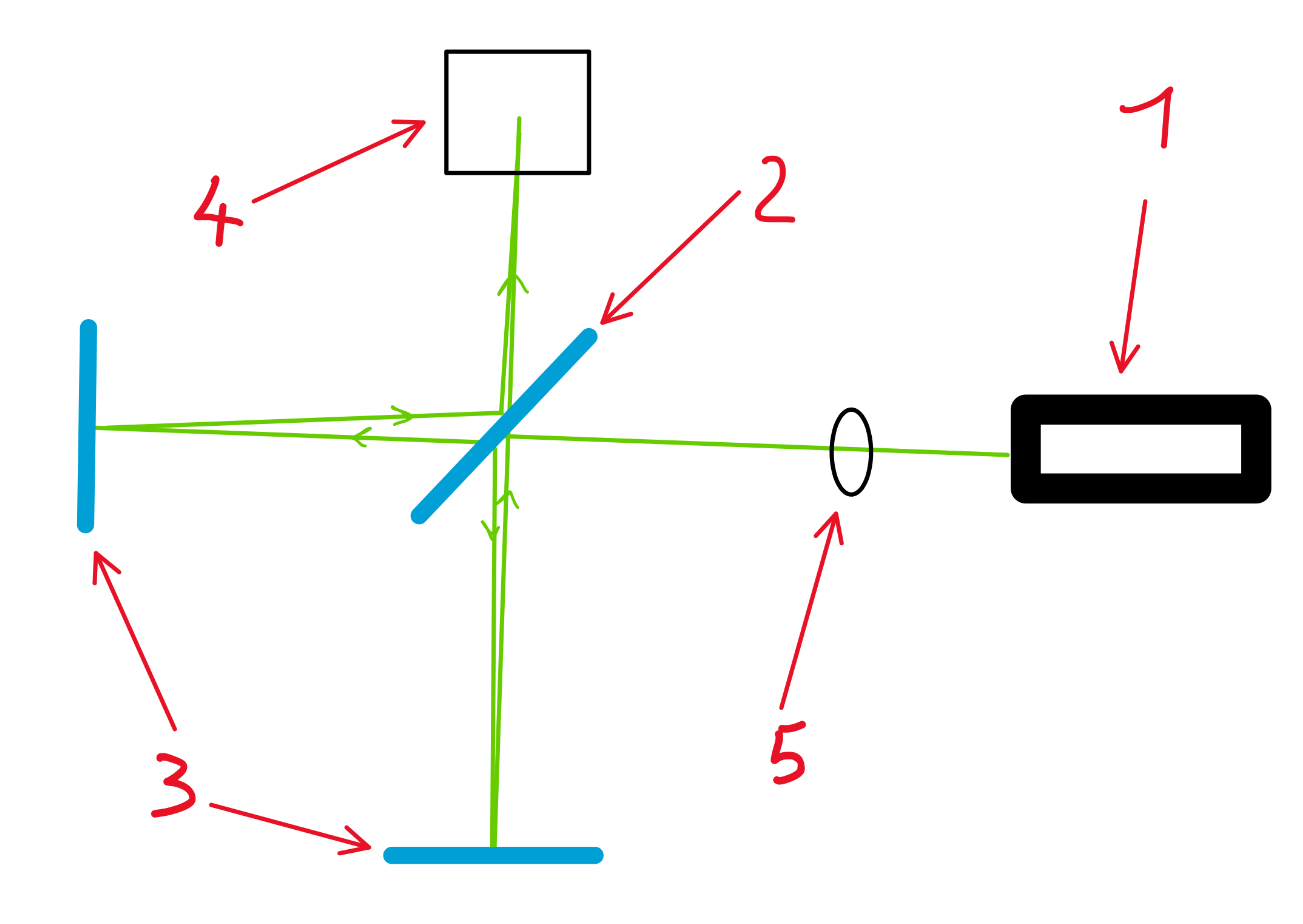
\includegraphics[width =0.75\textwidth]{./figures/aufbau_interferometer_skizze.jpg}
	\end{center}
	\caption[Skizze des Aufbaus des Michelson Interferometres] {Skizze des Aufbaus des
		Michelson Interferometres         \\
		1 \dots LASER                     \\
		2 \dots Beamsplitter              \\
		3 \dots Spiegel                   \\
		4 \dots Schirm mit Beugungsmuster \\
		5 \dots Linse
	}\label{fig:aufbau_interferometer_skizze}
\end{figure}

Der Beamsplitter entspricht dabei einem dünnen Glasplättchen mit einer
speziellen Beschichtung, durch die die Hälfte des Strahls refektiert und die
andere Hälfte durchgelassen wird. Das entsprechende Beugungsmuster am Schirm
entsteht dabei durch Interferenz der beiden Lichtstrahlen von den
unterschiedlichen Lichtarmen. Eine ebene Welle kann dabei in folgender Form
dargestellt werden:

\begin{equation}
	E(x, t)=E_0 \exp i(\omega t-k x)
\end{equation}

Dadurch kann die Lichtintensität folgend ausgedrückt werden:
\begin{equation}
	I=1 /{ }_4 c \varepsilon_0 E_0^2(1+\cos \Delta \varphi)
\end{equation}

Dabei entspricht $\Delta \varphi$ der Phasendifferenz, die sich aus dem
Unterschied der Weglängen $\Delta s=\left|s_1-s_2\right|$ nach folgender Formel
berechnet:
\begin{equation}
	\Delta \varphi=(2 \pi / \lambda) \Delta s
\end{equation}

Das Ringmuster im Interferenzbild kann dabei anhand folgenden Strahlengang in
\autoref{fig:aufbau_interferometer_skizze_demtroder} erklärt
werden.

\begin{figure}[H]
	\begin{center}
		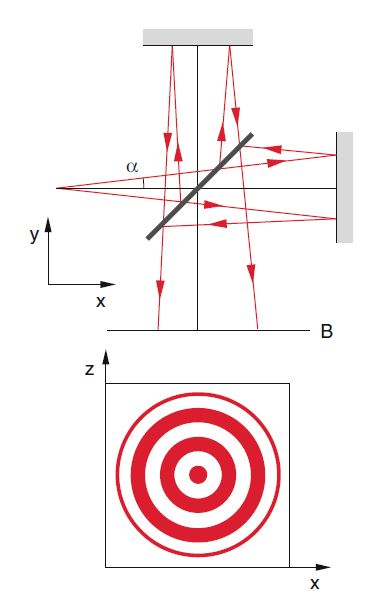
\includegraphics[width =0.3\textwidth]{./figures/linse_demtroder.jpg}
	\end{center}
	\caption[Skizze des Lichtwegs durch die Linse] {Skizze des Lichtwegs durch die Linse
		\cite{demtroderExperimentalphysik2014}
	}\label{fig:aufbau_interferometer_skizze_demtroder}
\end{figure}

Mithilfe des Interferometers können bereits sehr kleine Weglängenänderungen in
den Lichtarmen sichtbar gemacht werden. Aufgrund der Geometrie entspricht eine
Armlängenänderung die im Interferenzbild den Wechsel von einem
Interferenzmaximum zum nächsten entspricht, einer Änderung der halben
Wellenlänge, weil der Weg zwischen Beamsplitter und Spiegel insgesamt 2 mal
zurückgelegt wird.\cite{krennInterferenzUndPolarisation2023}

\section{Versuchsanordnung}\label{sec:versuchsanordnung}

Für alle Versuche wird als Lichtquelle ein LASER mit einer Wellenlänge
$\lambda$ von \SI{532}{\nano\meter} und einer Leistung von \SI{5}{\milli\watt}
verwendet. Der gesamte Versuch wird auf einem Breadboard aufgebaut, welches auf
einer gedämpften Steinplatte steht, um Erschütterungen besser ausgleichen zu
können. Dies wird noch genauer in \autoref{sec:diskussion} behandelt.
\subsection{Young'scher Doppelspalt, Beugungsgitter}

Der fertige Versuchsaufbau ist in \autoref{fig:aufbau_doppelspalt} sichtbar.
Die entsprechenden Nummerierungen entsprechen dabei den Justierungsschritten in
der Aufzählung.

\begin{enumerate}
	\item Zunächst wird der LASER am Breadboard parallel ausgerichtet. Dazu kann der
	      Blechschirm mit der Skala (5) verwendet werden. Zusätzlich kann damit der
	      Laserstrahl während dem Hantieren oder seine Reflexionen ausgeblockt werden.
	\item Nun werden die beiden Spiegel, wie in \autoref{fig:aufbau_doppelspalt}
	      sichtbar, aufgestellt, um den Laserstrahl auf den entsprechenden Lichtweg zu
	      lenken. Erneut ist die parallele Ausrichtung zu überprüfen.
	\item Nun wird mithilfe des entsprechenden Diahalters der Doppelspalt in den Lichtweg
	      gegeben. Durch den Doppelspalt entsteht eine Reflexion die auf den Spiegel
	      zurückgeworfen wird. Durch die Position dieser Reflexion auf den Spiegel kann
	      die parallele Ausrichtung des Aufbaus überprüft werden. Nun werden die genauen
	      Ausrichtungen der Spiegel und des LASERs durch die entsprechenden
	      Feinjustierungsschrauben so lange nachjustiert, bis die Positionen
	      übereinstimmen.
	\item Um die Entfernung zwischen Schirm und Doppelspalt zu maximieren, wird als
	      Schirm die Wand verwendet. Um die einzelnen Distanzen zwischen den
	      Beugungsmaxima besser bestimmen zu können, wird auf die Position des
	      Beugungsbilds ein Blatt Millimeterpapier geklebt.
\end{enumerate}

\begin{figure}[H]
	\begin{center}
		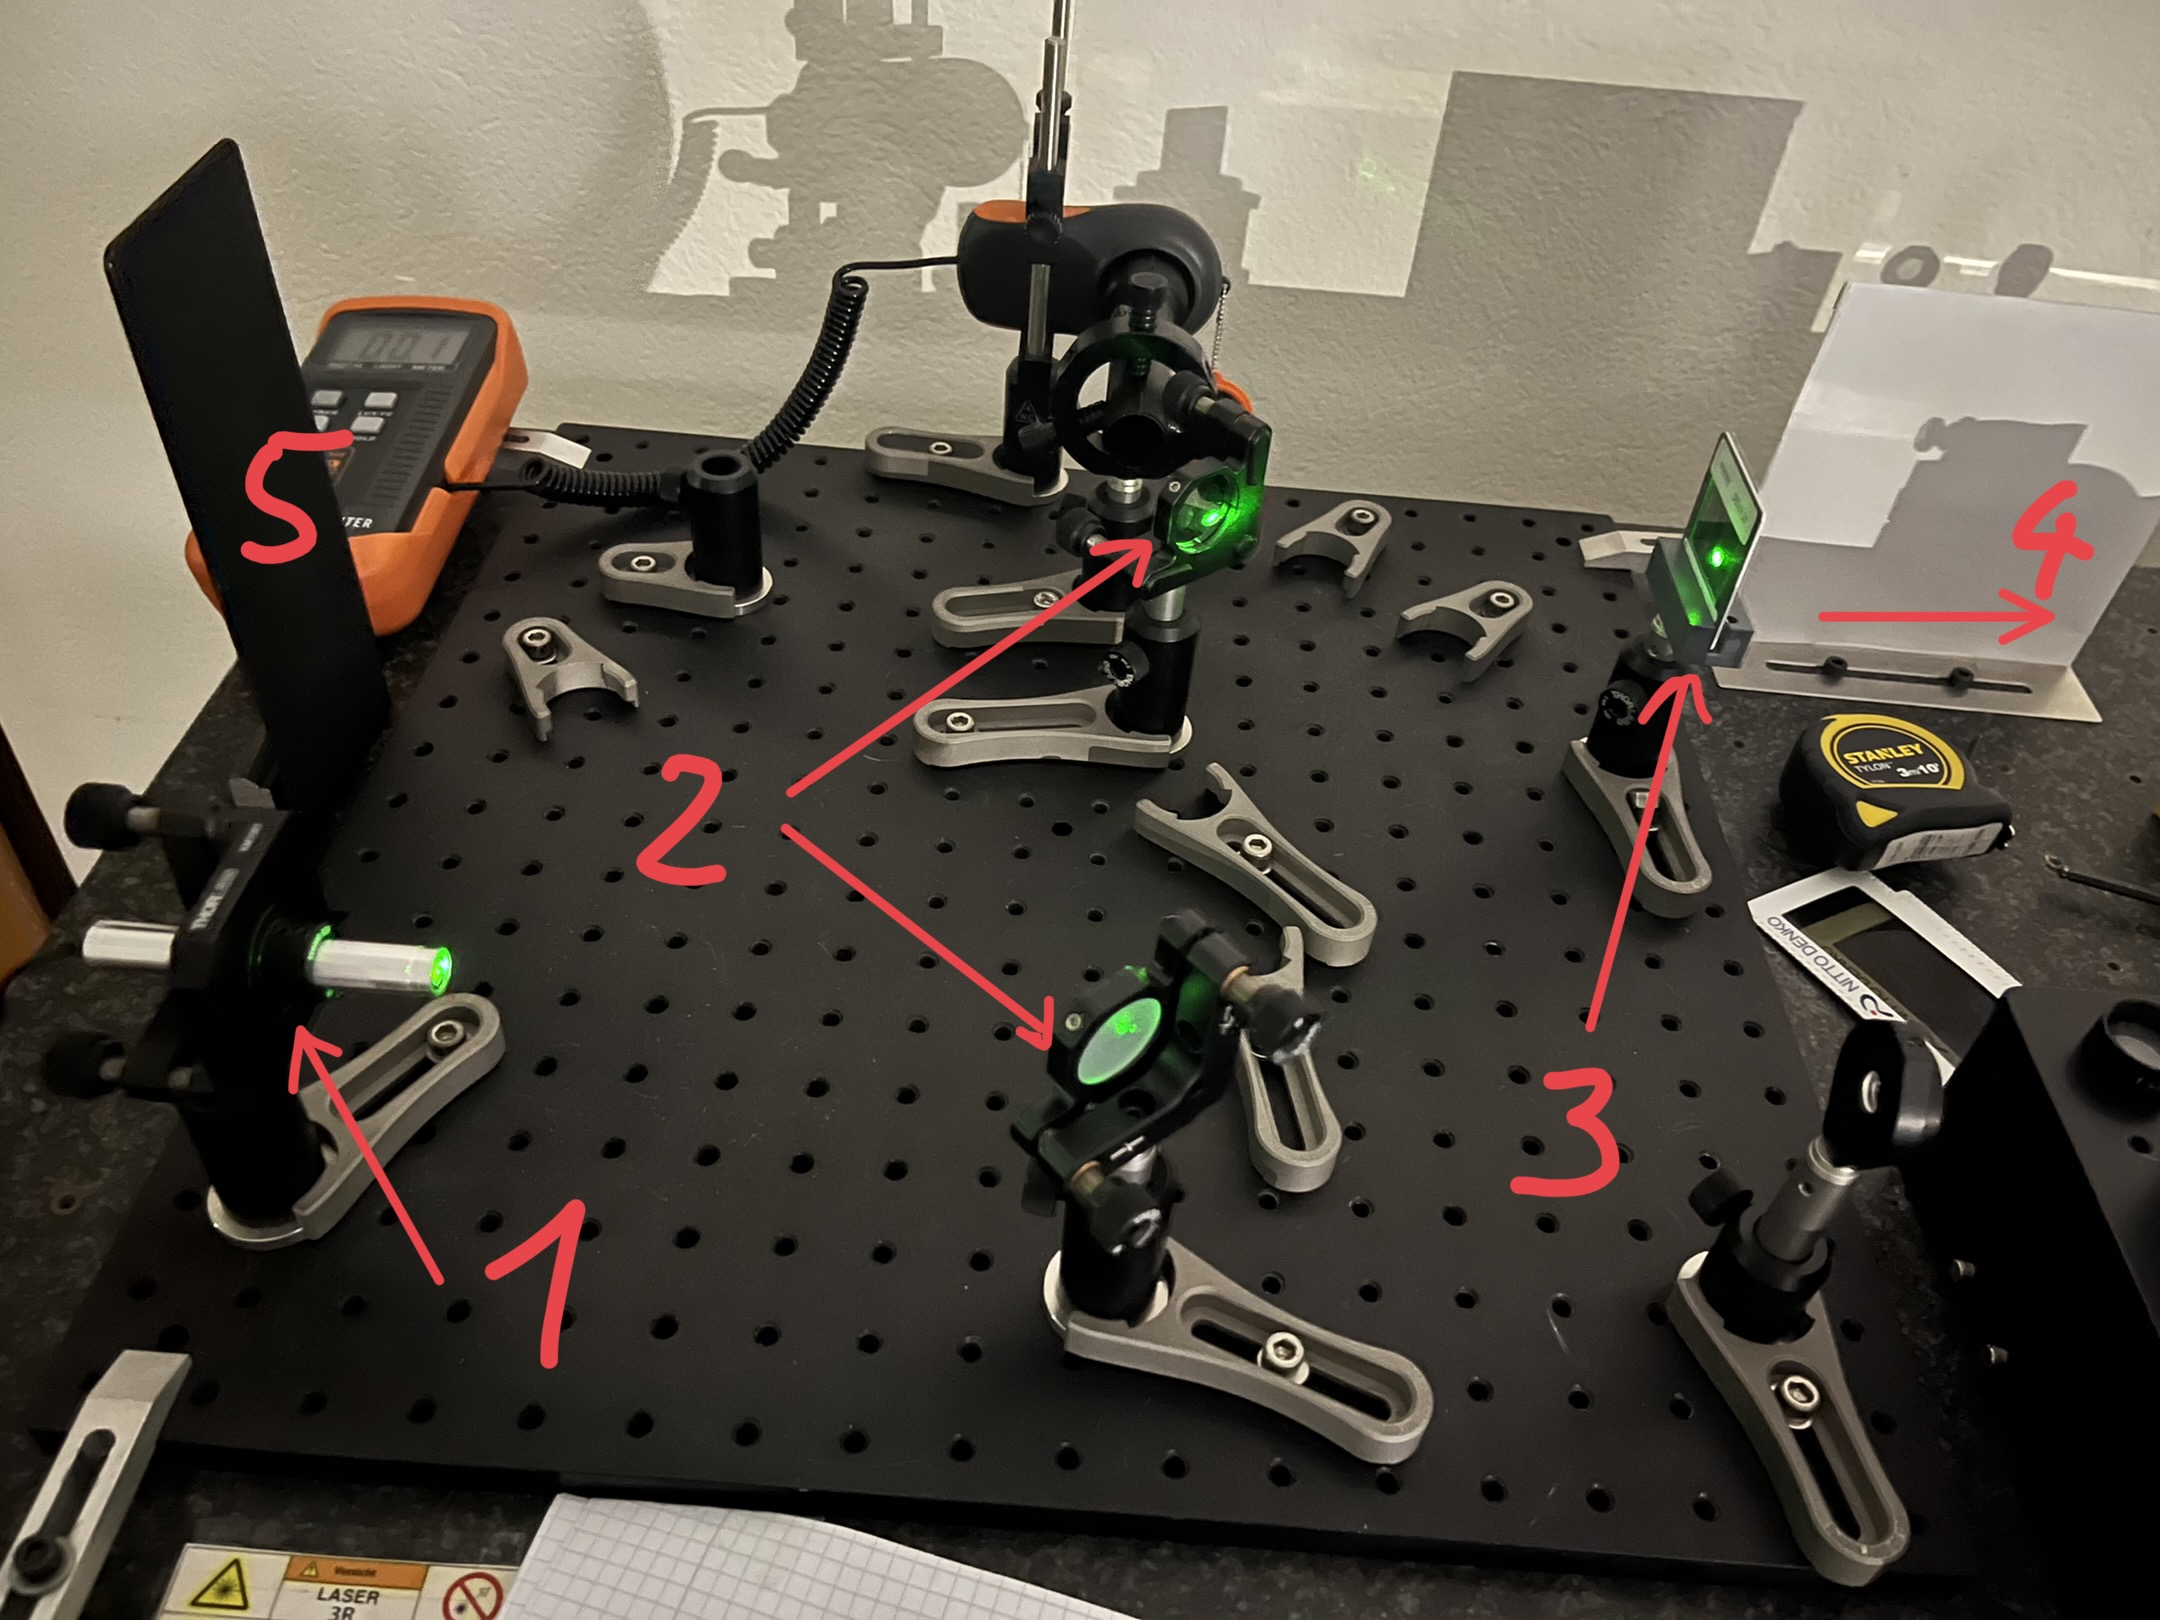
\includegraphics[width =0.75\textwidth]{./figures/aufbau_doppelspalt.jpg}
	\end{center}
	\caption[Versuchsaufbau für den Young'schen Doppelspalt und das Beugungsgitter] {
		Versuchsaufbau für den Young'schen Doppelspalt und das Beugungsgitter \\
		1 \dots LASER                                                         \\
		2 \dots Spiegel                                                       \\
		3 \dots Halterung mit Young'schen Doppelspalt oder dem Beugungsgitter \\
		4 \dots Schirm auf der Wand (nicht sichtbar)                          \\
		5 \dots Blechschirm mit Skala
	}\label{fig:aufbau_doppelspalt}
\end{figure}

\newpage

\subsection{Polarisation}

Der fertige Versuchsaufbau ist in \autoref{fig:aufbau_polarisation} sichtbar.
Die entsprechenden Nummerierungen entsprechen dabei den Justierungsschritten in
der Aufzählung.

\begin{enumerate}
	\item Zunächst wird wieder der LASER am Breadboard parallel ausgerichtet. Dabei kann
	      der Blechschirm mit der Skala, wie bereits erklärt, verwendet werden.
	\item Nun wird ein Spiegel, wie in \autoref{fig:aufbau_polarisation} sichtbar,
	      aufgestellt, um den Laserstrahl zum Photodetektor (3) zu lenken. Erneut ist die
	      parallele Ausrichtung zu überprüfen.
	\item Vor dem Photodetektor wird ein Rohr mithilfe einer entsprechenden Halterung
	      befestigt, um die Hintergrundbeleuchtung möglichst abzuschirmen.
	\item Um die entsprechende Lichtintensität ablesen zu können, wird das entsprechende
	      Messgerät mit dem Photosensor verbunden.
	\item Zwischen Photodetektor und Spiegel werden nun noch zwei Polarisationsfilter
	      gegeben, deren Orientierung mit einer Skala verbunden ist.
\end{enumerate}

\begin{figure}[H]
	\begin{center}
		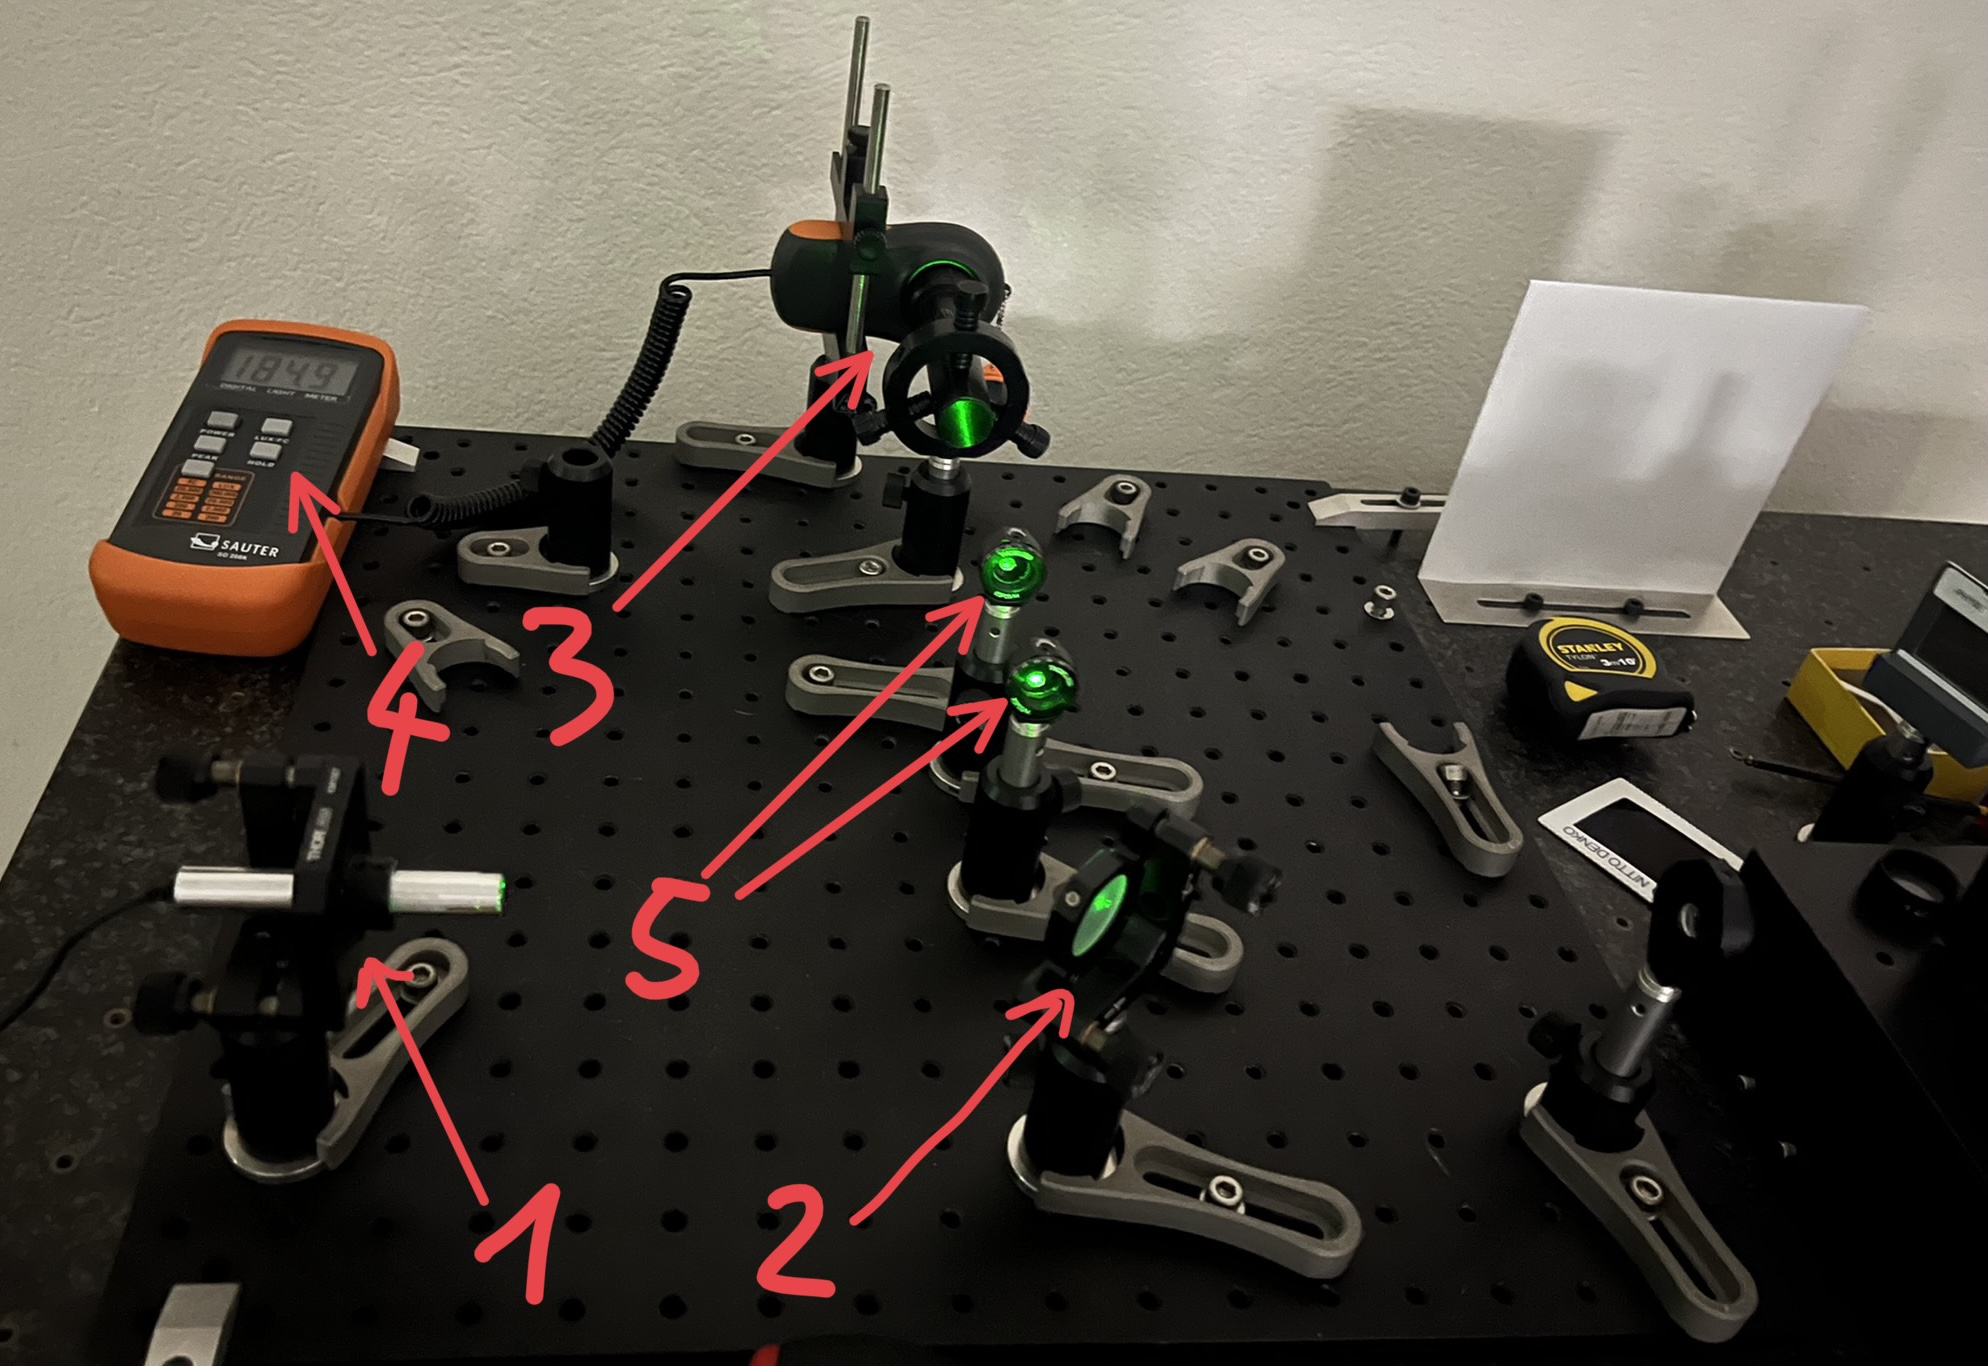
\includegraphics[width =0.75\textwidth]{./figures/aufbau_polarisation.jpg}
	\end{center}
	\caption[Versuchsaufbau für die Polarisation] { Versuchsaufbau für die Polarisation \\
		1 \dots LASER                       \\
		2 \dots Spiegel                     \\
		3 \dots Photodetektor mit Rohr      \\
		4 \dots Messgerät für Photosensor   \\
		5 \dots Polarisationsfilter
	}\label{fig:aufbau_polarisation}
\end{figure}

\subsection{Michelson Interferometer}

Der fertige Versuchsaufbau ist in \autoref{fig:aufbau_interferometer} sichtbar.
Die entsprechenden Nummerierungen entsprechen dabei den Justierungsschritten in
der Aufzählung. Der Hauptbestandteil des Interferometers befindet sich nicht
auf dem Breadboard, sondern auf der Platte daneben.

\begin{enumerate}
	\item Zunächst wird die Platte, auf der sich das Interferometer befindet so
	      befestigt, dass sie nicht mehr wackelt.
	\item Dann wird der LASER am Breadboard wieder parallel ausgerichtet, sodass dieser
	      auf den Beamsplitter trifft.
	\item Der Strahlteiler sorgt dafür, dass der halbe Lichtstrahl durchgelassen und die
	      andere Hälfte in einem Winkel von 90 ° abgelenkt wird.
	\item Nun Nun werden die beiden Spiegel so eingerichtet, dass das Licht zurück zum
	      Beamsplitter geworfen wird, wo es miteinander interferieren kann. Bei der
	      genauen Ausrichtung der Spiegel ist dabei darauf zu achten, dass sich diese im
	      90 ° Winkel zueinander befinden und beide Lichtwege ca. gleich lang sind.
	\item Am Schirm wird das Interferenzbild der beiden Laserstrahlen sichtbar. Die
	      genaue Position des einen Spiegels bzw. des LASERs muss nun so lange
	      feinjustiert werden, bis ein Interferenzmuster sichtbar wird.
	\item Um dafür zu sorgen, dass das Interferenzmuster ringförmig wird, wird eine Linse
	      in den Strahlengang vor den Beamsplitter gegeben.
	\item Mit dieser Halterung kann im späteren Verlauf ein Polarisationsfilter im
	      Strahlengang fixiert werden.
	\item Durch die Schraube und die entsprechende Übersetzung kann einer der beiden
	      Lichtwege um eine kleine Distanz verkürzt werden.
\end{enumerate}

\begin{figure}[H]
	\begin{center}
		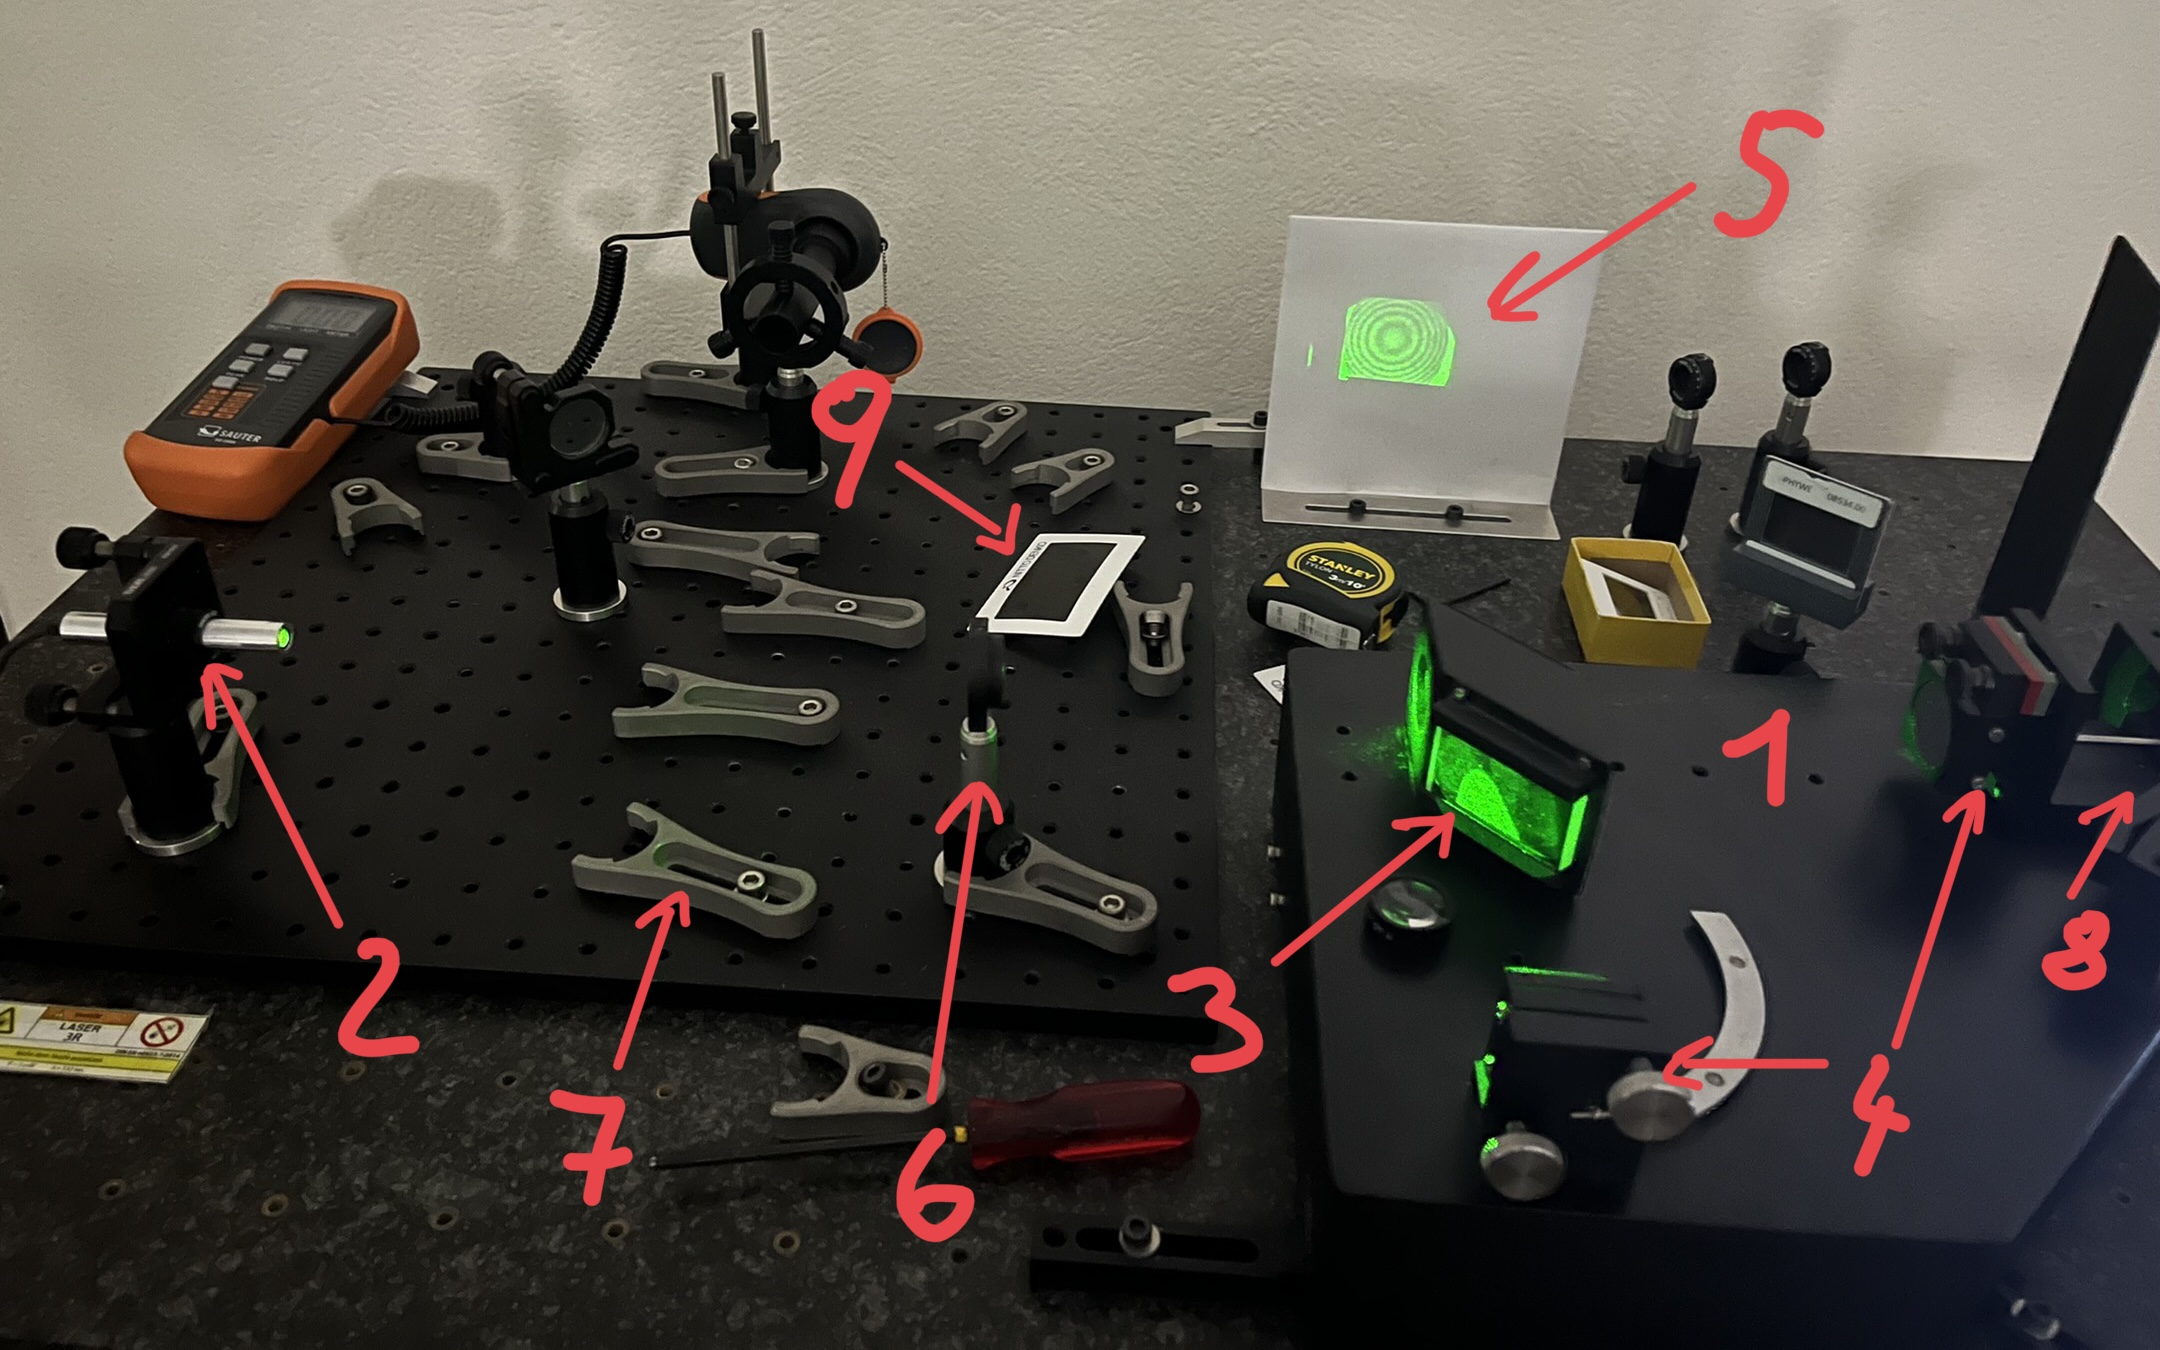
\includegraphics[width =0.75\textwidth]{./figures/aufbau_interferometer.jpg}
	\end{center}
	\caption[Versuchsaufbau für das Interferometer] { Versuchsaufbau für das Interferometer                                   \\
		1 \dots Platte für Interferometer                                       \\
		2 \dots LASER                                                           \\
		3 \dots Beamsplitter                                                    \\
		4 \dots Spiegel                                                         \\
		5 \dots Schirm                                                          \\
		6 \dots Linse                                                           \\
		7 \dots Halterung für Polarisationsfilter                               \\
		8 \dots Schraube für die Distanzänderung der Lichtarme (nicht sichtbar) \\
		9 \dots Polarisationsfolie                                              \\
	}\label{fig:aufbau_interferometer}
\end{figure}

\newpage

\section{Geräteliste}\label{sec:geraeteliste}

Für den Versuch werden die in \autoref{tab:gerate} aufgelisteten Geräte
verwendet.

\begin{table}[H]
	\begin{center}
		\caption{Verwendete Geräte
		}
		\begin{tblr}{cells={font=\footnotesize},colspec={lllll}}
			\textbf{Gerätetyp}         & \textbf{Hersteller} & \textbf{Typ}               & \textbf{Anmerkung}                \\
			LASER                      & ThorLabs            & CPS532-C2                  & $\lambda$ = \SI{532}{\nano\meter} \\
			Adapterring für LASER      & ThorLabs            & AD11NT                     &                                   \\
			Halterungsring für LASER   & ThorLabs            & KM100T                     &                                   \\
			Netzteil für LASER         & ThorLabs            & 973-579-7227               &                                   \\
			Spiegel                    & ThorLabs            & PF10-03-P01                & 2x                                \\
			Halterungsring für Spiegel & ThorLabs            & KM100                      & 2x                                \\
			Polarisationsfilter        & ThorLabs            & RSP05/M                    & 2x                                \\
			Polarisationsfolie         & NITTO DENKO         &                            & 2x                                \\
			Halterungsring für Linse   & ThorLabs            & FMP1/M                     &                                   \\
			Sammellinse                & ThorLabs            & f = \SI{40}{\milli\meter}  &                                   \\
			Zerstreulinse              & ThorLabs            & f = \SI{-16}{\milli\meter} &                                   \\
			Photosensor mit Messgerät  & Sauter              & S1152203                   &                                   \\
			Halterungsring Photosensor & selbstbau           &                            &                                   \\
			Abdeckrohr mit Halterung   & selbstbau           &                            &                                   \\
			Interferometeraufbau       & selbstbau           &                            &                                   \\
			Optical Posts              & ThorLabs            & TR40/M-JP-P5               & mehrmals                          \\
			Post Holder                & ThorLabs            & UPH40/M-P5                 & mehrmals                          \\
			Justierungsblech           &                     &                            &                                   \\
			Breadboard                 &                     &                            &                                   \\
			Millimeterpapier           &                     &                            &                                   \\
		\end{tblr}\label{tab:gerate}
	\end{center}
\end{table}

\section{Versuchsdurchführung und Messergebnisse}\label{sec:versuchsdurchfuehrung_messergebnisse}

\subsection{Young'scher Doppelspalt, Beugungsgitter}

Zunächst muss der Versuchsaufbau, wie bereits in
\autoref{sec:versuchsanordnung} beschrieben durchgeführt werden. Nun werden der
Reihe nach die 4 verschiedenen Doppelspalt in den Versuchsaufbau gegeben. Die
entsprechenden Abmessungen der Doppelspalte sind dabei in
\autoref{tab:masse_doppelspalt} sichtbar. Die entstehenden Beugungsmuster der
einzelnen Doppelspalte werden dabei fotografiert und sind im Folgenden
\autoref{fig:beugungsbild_spalt1} - \ref{fig:beugungsbild_spalt4} sichtbar. Um
die entsprechenden Distanzen im Beugungsbild besser messen zu können, werden
die so generierten Fotos bezüglich der Pixelpositionen genau ausgewertet, wie
genauer in \autoref{sec:auswertung} erklärt. Als Referenz dazu dient das im
Hintergrund befindliche Millimeterpapier.

\begin{table}[H]
	\begin{center}
		\caption[Maße der Doppelspalte]{Maße der Doppelspalte mit implizit gegebener
			Unsicherheit \cite{krennInterferenzUndPolarisation2023} \\
			$S_i$ \dots i-ter Doppelspalt                           \\
			$B$ \dots Spaltbreite in mm                             \\
			$D$ \dots Spaltabstand in mm
		}
		\begin{tblr}{cells={font=\footnotesize},colspec={lllll}}
			\textbf{} & $B$ / mm & $D$ / mm \\
			$S_1$     & 0.10     & 1.00     \\
			$S_2$     & 0.10     & 0.50     \\
			$S_3$     & 0.10     & 0.25     \\
			$S_4$     & 0.20     & 0.25     \\
		\end{tblr}\label{tab:masse_doppelspalt}
	\end{center}
\end{table}

Für das Fotografieren muss mit der Hintergrundbeleuchtung experimentiert
werden, damit die Millimetereinteilung sichtbar ist, jedoch auch die schwachen
Beugungsordnungen noch erkannt werden können. Auch muss darauf geachtet werden,
beim Aufnehmen der Fotos möglichst nahe am Beugungsbild zu sein, aber keinen
Zoom der Kamera zu verwenden, um eine mögliche Verzerrung auf den Bildern zu
vermeiden. Auch sollten alle Fotos aus der gleichen Perspektive aufgenommen
werden. Dazu wird ein kleines Gerüst gebaut, um immer die gleiche
Kameraposition zu treffen.

\begin{figure}[H]
	\begin{center}
		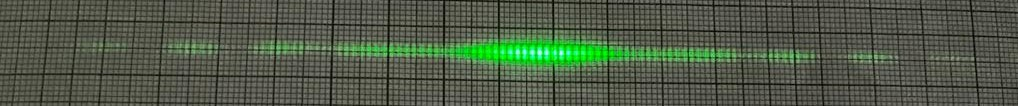
\includegraphics[width =\textwidth]{./figures/beugungsbild_spalt1_neu.jpg}
	\end{center}
	\caption{Erzeugtes Beugungsbild für Spalt 1 mit einer Spaltbreite von \SI{0.1}{\milli\meter} und einem Spaltabstand
		von \SI{1}{\milli\meter}
	}
	\label{fig:beugungsbild_spalt1}
\end{figure}

\begin{figure}[H]
	\begin{center}
		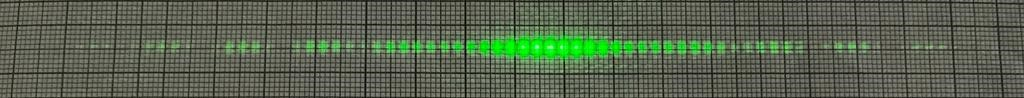
\includegraphics[width =\textwidth]{./figures/beugungsbild_spalt2_neu.jpg}
	\end{center}
	\caption{Erzeugtes Beugungsbild für Spalt 2 mit einer Spaltbreite von \SI{0.1}{\milli\meter} und einem Spaltabstand
		von \SI{0.5}{\milli\meter}
	}
	\label{fig:beugungsbild_spalt2}
\end{figure}

\begin{figure}[H]
	\begin{center}
		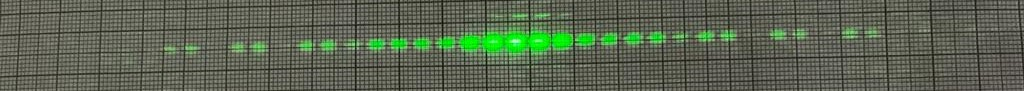
\includegraphics[width =\textwidth]{./figures/beugungsbild_spalt3_neu.jpg}
	\end{center}
	\caption{Erzeugtes Beugungsbild für Spalt 3 mit einer Spaltbreite von \SI{0.1}{\milli\meter} und einem Spaltabstand
		von \SI{0.25}{\milli\meter}
	}
	\label{fig:beugungsbild_spalt3}
\end{figure}

\begin{figure}[H]
	\begin{center}
		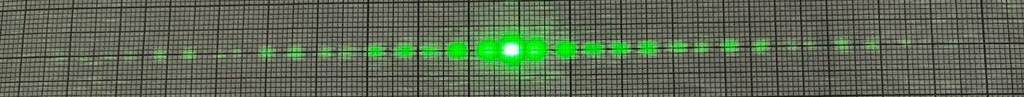
\includegraphics[width =\textwidth]{./figures/beugungsbild_spalt4_neu.jpg}
	\end{center}
	\caption{Erzeugtes Beugungsbild für Spalt 4 mit einer Spaltbreite von \SI{0.2}{\milli\meter} und einem Spaltabstand
		von \SI{0.25}{\milli\meter}
	}
	\label{fig:beugungsbild_spalt4}
\end{figure}



% \begin{figure}[H]
% 	\captionbox{Erzeugtes Beugungsbild für Spalt 1 mit einer Spaltbreite von \SI{0.1}{\milli\meter} und einem Spaltabstand
% 		von \SI{1}{\milli\meter}\label{fig:beugungsbild_spalt1}}{
% 		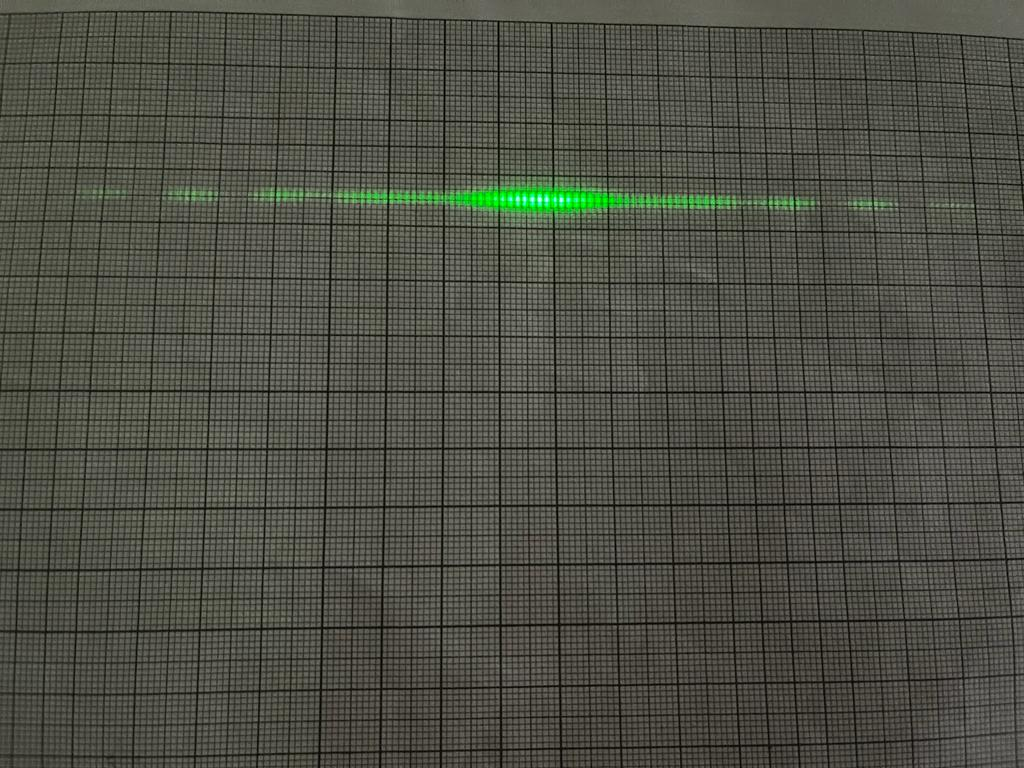
\includegraphics[width =.45\textwidth]{./figures/beugungsbild_spalt1.jpg} } \hfill
% 	\captionbox{Erzeugtes Beugungsbild für Spalt 2 mit einer Spaltbreite von \SI{0.1}{\milli\meter} und einem Spaltabstand
% 		von \SI{0.5}{\milli\meter}\label{fig:beugungsbild_spalt2}}{
% 		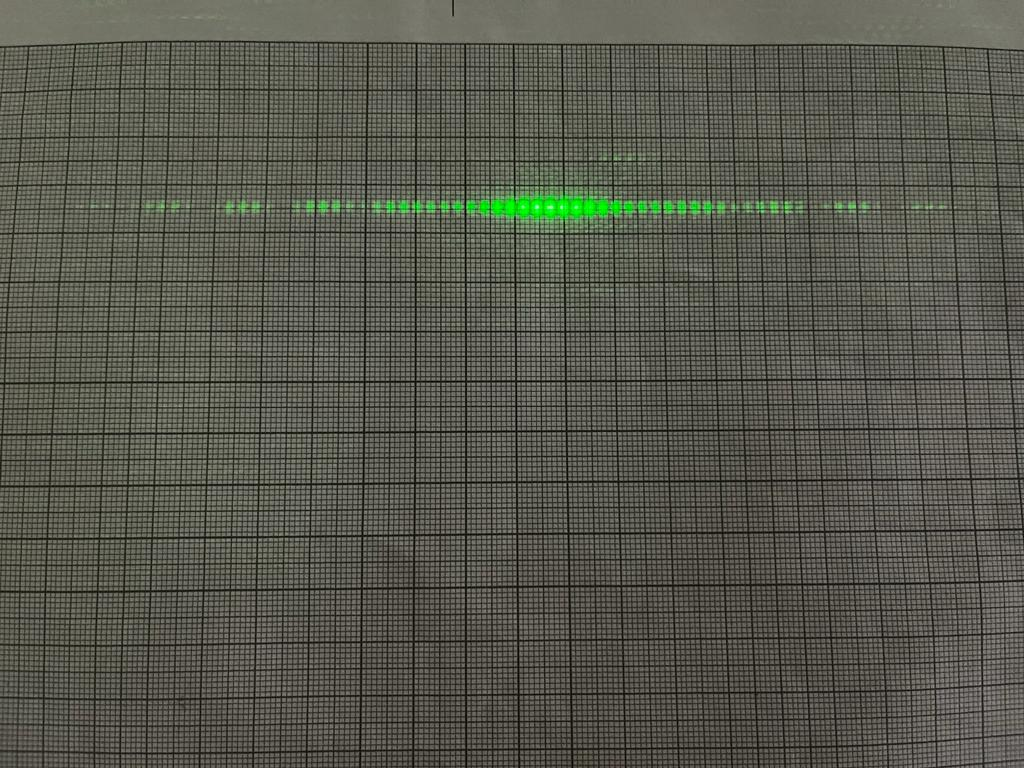
\includegraphics[width =.45\textwidth]{./figures/beugungsbild_spalt2.jpg}
% 	}

% 	\captionbox{Erzeugtes Beugungsbild für Spalt 3 mit einer Spaltbreite von
% 		\SI{0.1}{\milli\meter} und einem Spaltabstand von
% 		\SI{0.25}{\milli\meter}\label{fig:beugungsbild_spalt3}}{
% 		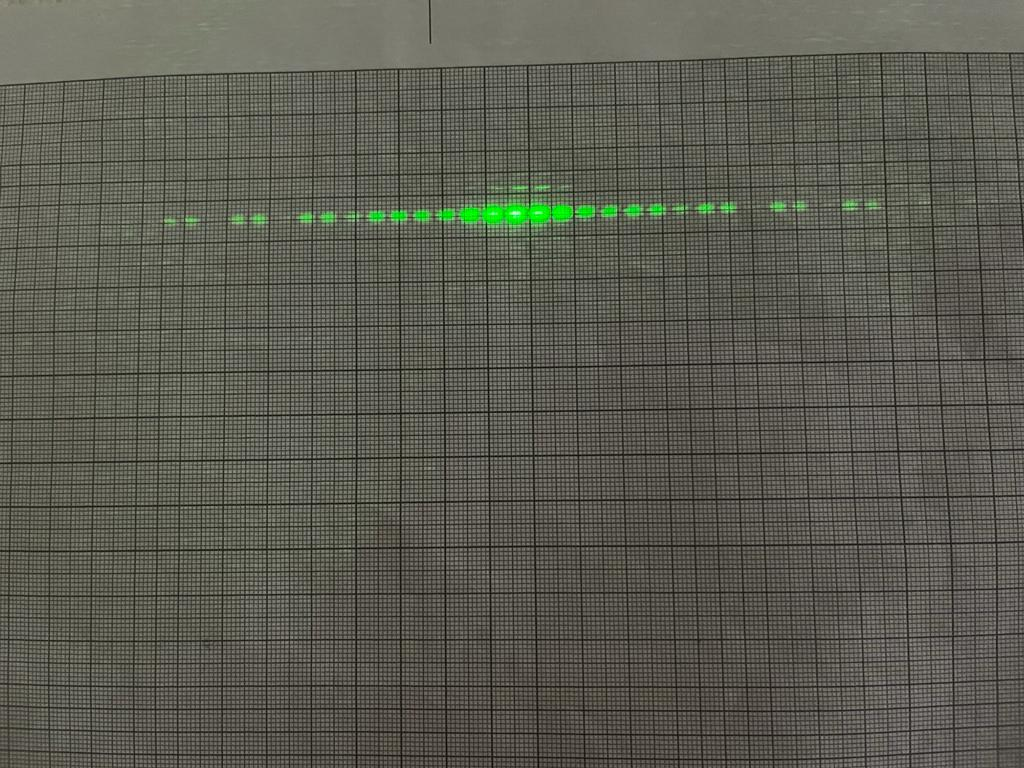
\includegraphics[width =.45\textwidth]{./figures/beugungsbild_spalt3.jpg} }
% 	\hfill \captionbox{Erzeugtes Beugungsbild für Spalt 4 mit einer Spaltbreite von
% 		\SI{0.2}{\milli\meter} und einem Spaltabstand von
% 		\SI{0.25}{\milli\meter}\label{fig:beugungsbild_spalt4}}{
% 		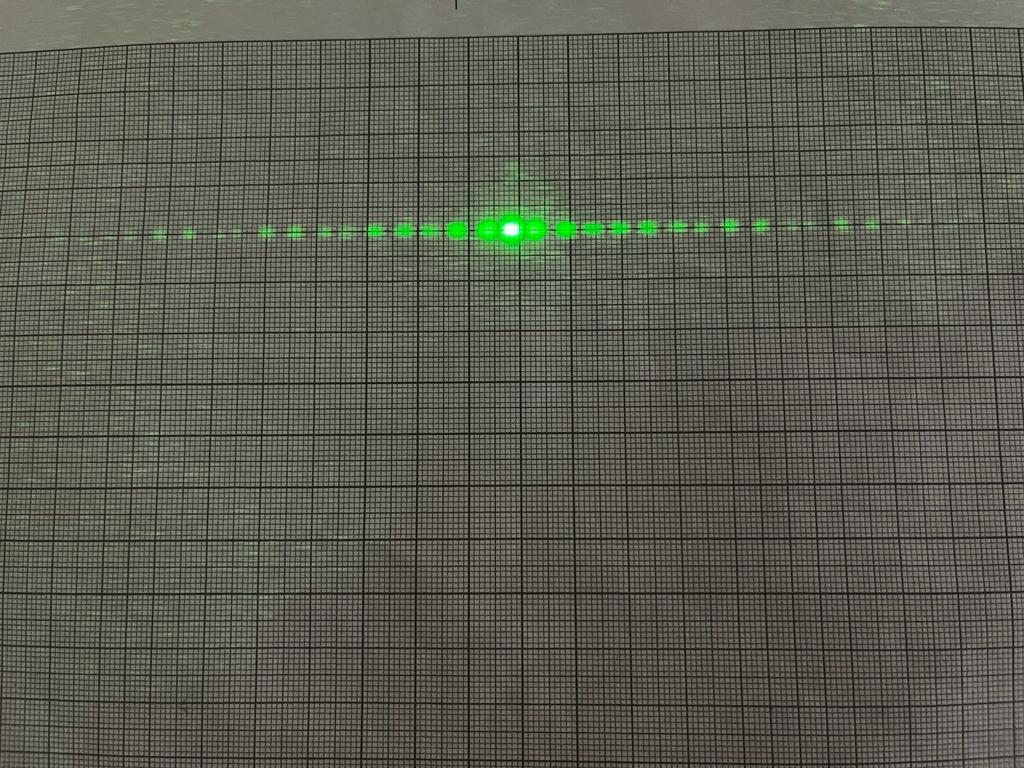
\includegraphics[width =.45\textwidth]{./figures/beugungsbild_spalt4.jpg} }
% \end{figure}

Nun wird die Abdeckung mit den Doppelspalten durch ein Beugungsgitter, also
viele, eng beieinander liegende Spalte ersetzt. Das so erzeugte Beugungsbild
ist in \autoref{fig:beugungsbild_gitter} sichtbar.

\begin{figure}[H]
	\begin{center}
		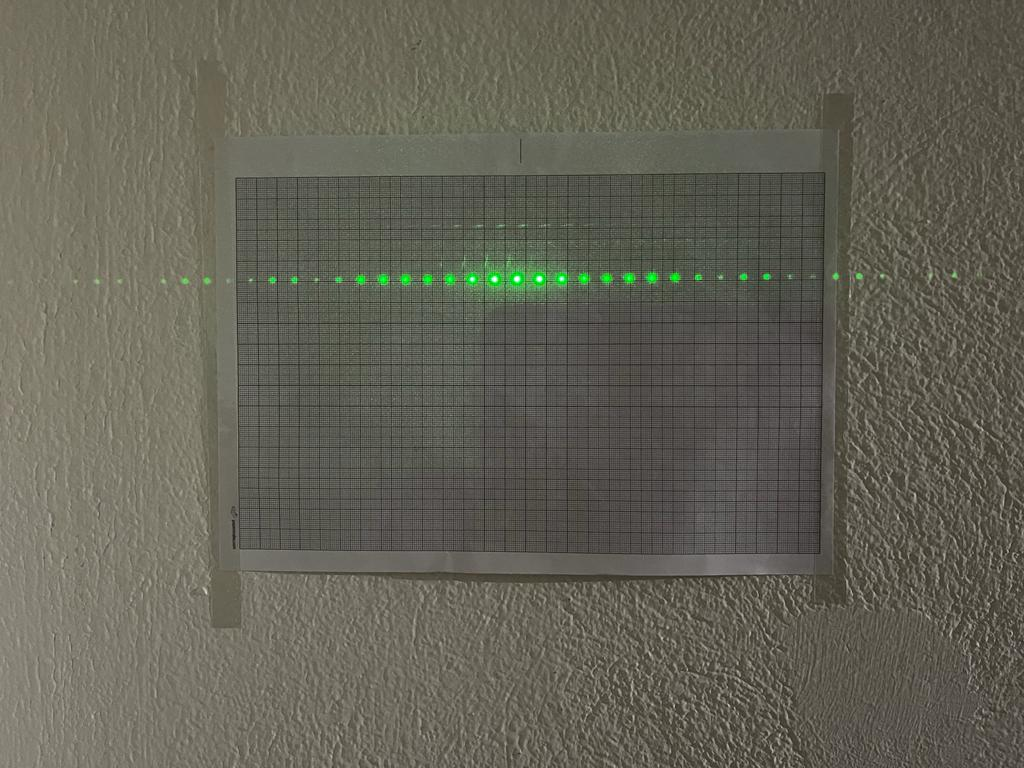
\includegraphics[width =0.5\textwidth]{./figures/beugungsbild_gitter.jpg}
	\end{center}
	\caption[ Erzeugtes Beugungsbild für das Beugungsgitter] { Erzeugtes Beugungsbild für das
		Beugungsgitter
	}\label{fig:beugungsbild_gitter}
\end{figure}

\subsection{Polarisation}

Zunächst muss der Versuchsaufbau, wie bereits in
\autoref{sec:versuchsanordnung} beschrieben durchgeführt werden.

An beiden Polarisationsfiltern wird zunächst die 0-Position eingestellt und
diese in den Aufbau gegeben. Im Verlauf des Versuchs sollen nun die
Polarisationsebenen zueinander verdreht werden. Dazu bleibt ein
Polarisationsfilter konstant in der gleichen Ausrichtung. Der andere
Polarisationsfilter wird nun kontinuierlich weitergedreht und der abgelesene
Skalenwert, sowie die gemessene Helligkeit in Lux am entsprechenden
Photodetektor notiert, was in \autoref{tab:werte_polarisation} sichtbar ist. Am
Messgerät ist dabei zu beachten, dass der kleinst mögliche Messbereich gewählt
wird. Die Unsicherheit des Winkel ist dabei so groß gewählt, weil der genaue
Winkel recht schwer zu bestimmen war. Auch ist darauf zu achten, die
Raumbeleuchtung möglichst abzudunkeln, um die Messung dadurch nicht zu
Verfälschen.

\begin{table}[H]
	\caption{Diese Tabelle beinhaltet die gemessenen Beleuchtungsstärke $E_v$ 
  bei verschiedenen Winkel $\phi$ zwischen den Polarisatoren. Als Lichtquelle dient 
  dabei einem LASER.}\label{tab:werte_polarisation}
	\centering
	\begin{tblr}{cells={font=\tiny},row{1}={font=\mathversion{bold}\footnotesize},rowsep=0pt,colspec={S[table-format=3.0(1)]S[table-format=3.1(3)e1]}}
{{{$\phi$ / \si{\degree}}}} & {{{$E_v$ / \si{\lux}}}}\\
0(2) & 3(10)\\
10(2) & 1(10)\\
20(2) & 12(10)\\
30(2) & 44(10)\\
40(2) & 108(10)\\
50(2) & 2.3(10)e+02\\
60(2) & 3.3(10)e+02\\
70(2) & 4.7(10)e+02\\
80(2) & 5.8(10)e+02\\
90(2) & 6.4(10)e+02\\
100(2) & 6.3(10)e+02\\
110(2) & 5.6(10)e+02\\
120(2) & 4.6(10)e+02\\
130(2) & 2.3(10)e+02\\
140(2) & 194(10)\\
150(2) & 105(10)\\
160(2) & 48(10)\\
170(2) & 19(10)\\
180(2) & 3(10)\\
190(2) & 0(10)\\
200(2) & 8(10)\\
210(2) & 39(10)\\
220(2) & 99(10)\\
230(2) & 2.1(10)e+02\\
240(2) & 3.5(10)e+02\\
250(2) & 4.5(10)e+02\\
260(2) & 5.7(10)e+02\\
270(2) & 6.2(10)e+02\\
280(2) & 6.0(10)e+02\\
290(2) & 5.3(10)e+02\\
300(2) & 4.2(10)e+02\\
310(2) & 2.9(10)e+02\\
320(2) & 183(10)\\
330(2) & 99(10)\\
340(2) & 42(10)\\
350(2) & 17(10)\\
360(2) & 2(10)\\
7(2) & 0(10)\\
\end{tblr}

\end{table}

Zusätzlich wird auch der Intensitätswert ohne Polarisationsfilter $E_{v_0}$, mit nur
einem Filter $\frac{E_{v_0}}{2}$ und der Winkel  $\phi|_{E_v=0}$ bestimmt, an dem, laut Messgerät, kein Licht durch
den Aufbau gelangt, gemessen und notiert.

\begin{enumerate}
	\item $E_{v_0}=\SI{1170(100)}{\lux}$
	\item $\frac{E_{v_0}}{2}=\SI{765(100)}{\lux}$
	\item $\phi|_{E_v=0}=\SI{7(3)}{\degree}$
\end{enumerate}

Nun wird noch ein dritter Polarisator in Form einer Polarisationsfolie in den
Strahlengang gehalten durch den eigentlich keine Intensität gelangt. Dabei
werden folgende Werte erzeugt:

\begin{enumerate}
	\item $\tilde{E}_v|_{\phi\approx\SI{90}{\degree}}=\SI{0.0}{\lux}$
	\item $\tilde{E}_v|_{\phi\approx\SI{45}{\degree}}=\SI{35.3}{\lux}$
	\item $\tilde{E}_v|_{\phi\approx\SI{22}{\degree}}=\SI{17.8}{\lux}$
\end{enumerate}

Dabei sei angemerkt, dass nur so wenig Werte angegeben wurden, weil hier keine
Gradmessung möglich war und der entsprechende Winkel nur geschätzt werden
konnte.

\subsection{Michelson Interferometer}

Zunächst muss der Versuchsaufbau, wie bereits in
\autoref{sec:versuchsanordnung} beschrieben durchgeführt werden.

Nachdem das Interferometer fertig aufgebaut und justiert ist, wird die Linse
vor dem Beamsplitter aufgestellt. Dadurch ergeben sich nach dem LASER
verschiedene Lichtwege und damit verschiedene Weglängenänderungen, wie bereits
in \autoref{sec:Grund} erwähnt, wodurch das Ringförmige Interferenzmuster
zustandekommt.

Aufgrund des Aufbaus des Interferometers hat der andere Strahl der den
Beamsplitter verlässt eine andere Orientierung der Interferenzmuster. Das
bedeutet, dass der Ring, welcher an einen Ausgang durch konstruktive
Interferenz hell erscheint, am anderen Ausgang ein Minimum darstellt. Dies
könnte optimal mithilfe eines zweiten Strahlteilers gezeigt werden. Da dieser
nicht zur Verfügung war wurde das entsprechende Interfenzmuster mit einem
gelochten Papier betrachtet, welches als Lochblende verwendet wird, wie in
\autoref{fig:beugungsbild_lochblende} sichtbar.

\begin{figure}[H]
	\begin{center}
		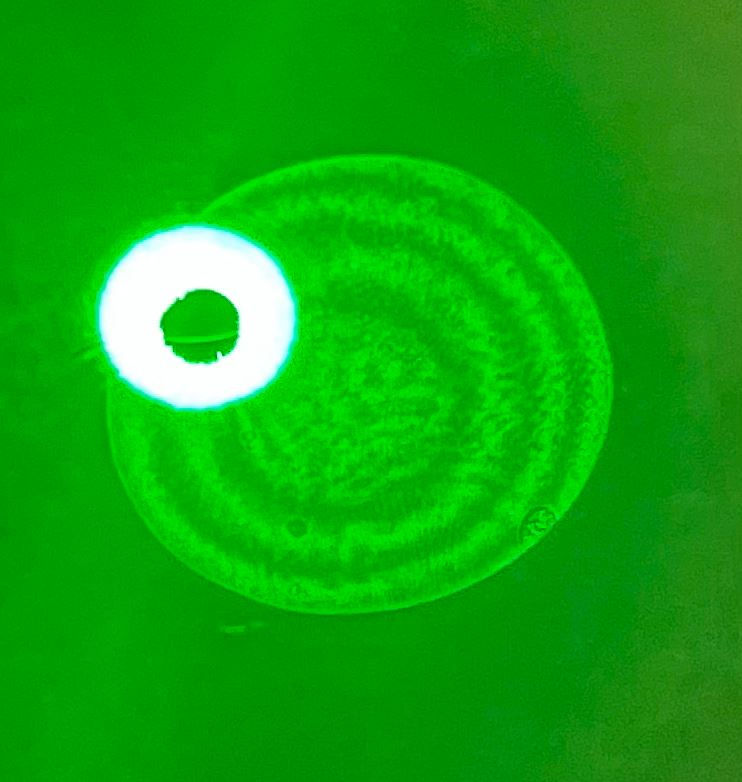
\includegraphics[width =0.5\textwidth]{./figures/Blende.JPG}
	\end{center}
	\caption[Sichtbares Interferenzmuster durch die Lochblende] { Sichtbares
		Interferenzmuster durch die Lochblende
	}\label{fig:beugungsbild_lochblende}
\end{figure}

Nun wird Die Länge eines Lichtarms Verändert, was ein scheinbares Wandern der
Interferenzringe mit sich bringt. Um die genaue Weglängenänderung bestimmen zu
können, ist ein Übersetzungsarm mit der Mykrometerschraube verbunden, wodurch
die genaue Distanz bestimmt werden kann. Dabei wird auf das Zentrum des
Interfenzmusters geachtet und immer die Weglänge bestimmt, damit 10
Interfenzmuster das Zentrum durchlaufen. Die entsprechenden Werte sind in
\autoref{tab:werte_interferometer} aufgelistet.

\begin{table}[H]
	\caption{Diese Tabelle beinhaltet Werte vom Michelson-Interferometer bei
  unterschiedlichen optischen Armlängen. Beim Varieren der Armlänge sind die Abstände 
$s$ auf dem Mikrometerschraube abgelesen worden und die dabei durchschrittenen Maxima 
$N$ gezählt worden.}\label{tab:werte_interferometer}
	\centering
	\begin{tblr}{cells={font=\footnotesize},row{1}={font=\mathversion{bold}\footnotesize},colspec={S[table-format=3.1(1)]S[table-format=2.1(1)]}}
{{{$N$ / 1}}} & {{{$s$ / \si{\milli\meter}}}}\\
10.0(0) & 1.0(0)\\
20.0(0) & 2.5(0)\\
30.0(0) & 4.0(0)\\
40.0(0) & 5.5(0)\\
50.0(0) & 7.0(0)\\
60.0(0) & 9.0(0)\\
70.0(0) & 10.0(0)\\
80.0(0) & 12.0(0)\\
90.0(0) & 13.5(0)\\
100.0(0) & 15.0(0)\\
110.0(0) & 16.5(0)\\
120.0(0) & 18.0(0)\\
130.0(0) & 20.0(0)\\
140.0(0) & 21.0(0)\\
150.0(0) & 22.5(0)\\
160.0(0) & 24.0(0)\\
170.0(0) & 25.5(0)\\
\end{tblr}

\end{table}

Bezüglich der Stabilität des Interferenzbildes wird klar ersichtlich, dass
dieses sehr sensitiv auf eventuelle Schwingungen reagiert. Dies kann durch
Erschütterungen beobachtet werden. Besser sichtbar wird dies durch vorsichtiges
Rütteln des Sockels. Um die starke Sensitivität auf Erschütterungen sichtbar zu
machen, wird mithilfe des Handys Musik abgespielt, während dieses auf den
Sockel des Interferoeters gelegt wird. So kann beobachtet werden, wie Störungen
im Interferenzmuster im Takt der Musik auftreten.

Ein weiterer Aspekt, der Beobachtet werden kann, ist die Änderung des
Ausbreitungsmedium in einem der Lichtarme. Dazu wird die Luft in einem der
Lichtarme mithilfe eines Feuerzeugs erhitzt. Dadurch wird durch die so
entstehenden Luftwirbel kein deutliches Interferenzmuster mehr sichtbar.

Nun wird die Sammellinse entfernt und eine Zerstreulinse zwischen Beamsplitter
und Schirm gegeben. Dadurch wird das streifenförmige Interferenzmuster am
Schirm sichtbar, siehe \autoref{fig:interferometer_linse}.

\begin{figure}[H]
	\begin{center}
		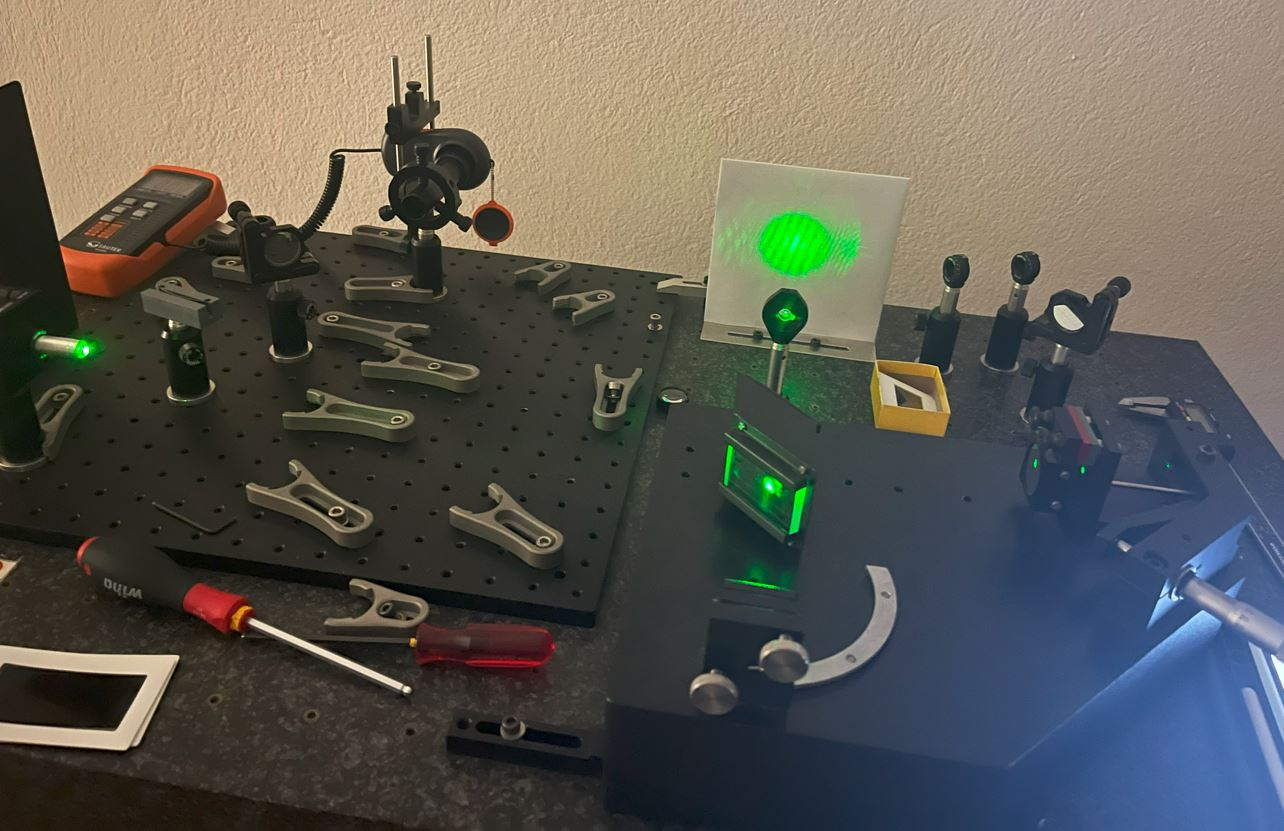
\includegraphics[width =0.75\textwidth]{./figures/Interferometer_linse.JPG}
	\end{center}
	\caption[Sichtbares Interferenzmuster mit der Linse nach dem Beamsplitter] { Sichtbares
		Interferenzmuster mit der Linse nach dem Beamsplitter
	}\label{fig:interferometer_linse}
\end{figure}

Es wird klar ersichtlich, dass sich ein streifenförmiges Interferenzmuster
bildet. Dieses lässt sich durch konstruktive und destruktive Interferenz des
Laserstrahls erklären.

Nun werden 2 Polarisationsfolien in die beiden Lichtarme gegeben, wie in
\autoref{fig:interferometer_polarisation} ersichtlich.

\begin{figure}[H]
	\centering
	\begin{subfigure}{.45\linewidth}
		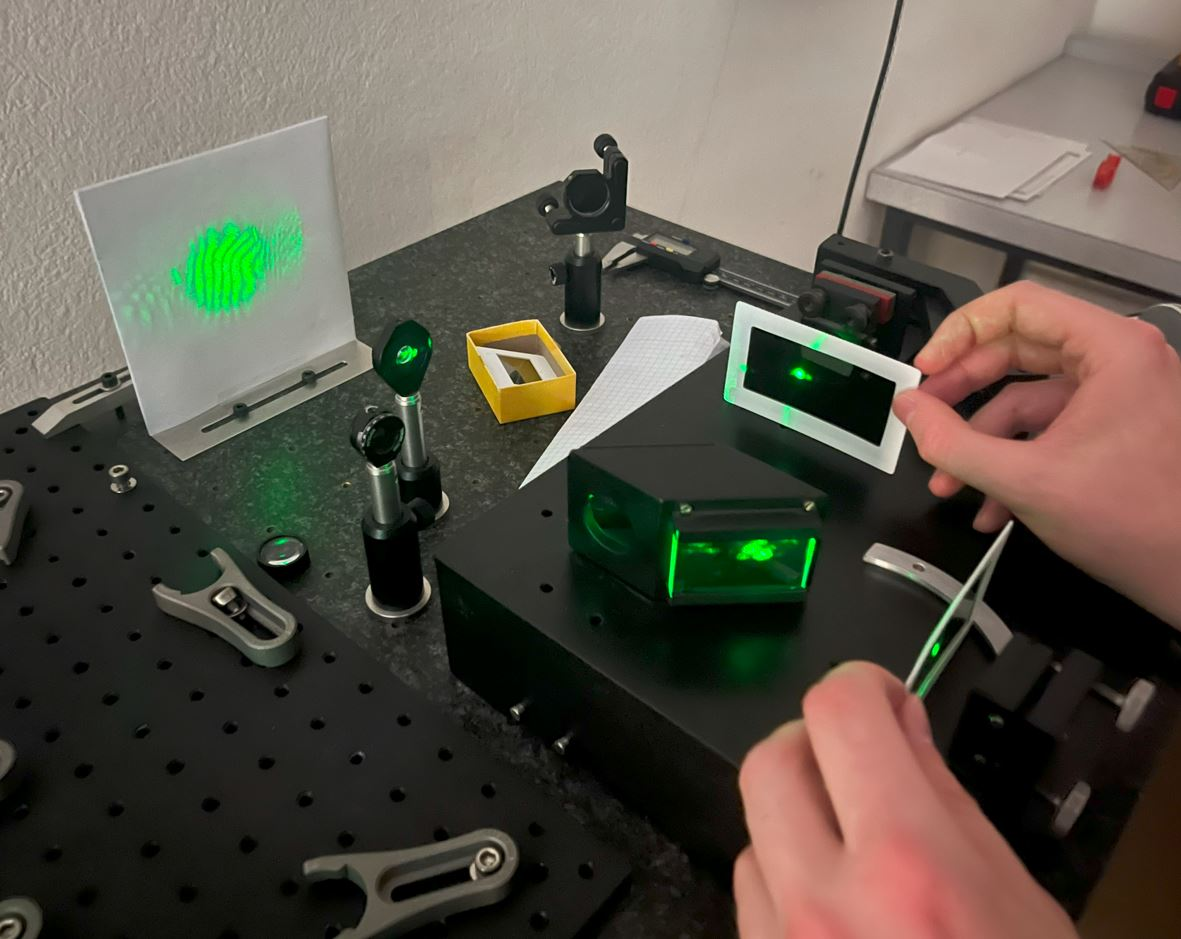
\includegraphics[width=\textwidth]{./figures/Interferometer_polarisation_parallel.JPG}
		\caption{Parallele Ausrichtung der Polarisationsfilter
		}\label{fig:interferometer_polarisation_parallel}
	\end{subfigure}
	\begin{subfigure}{.45\linewidth}
		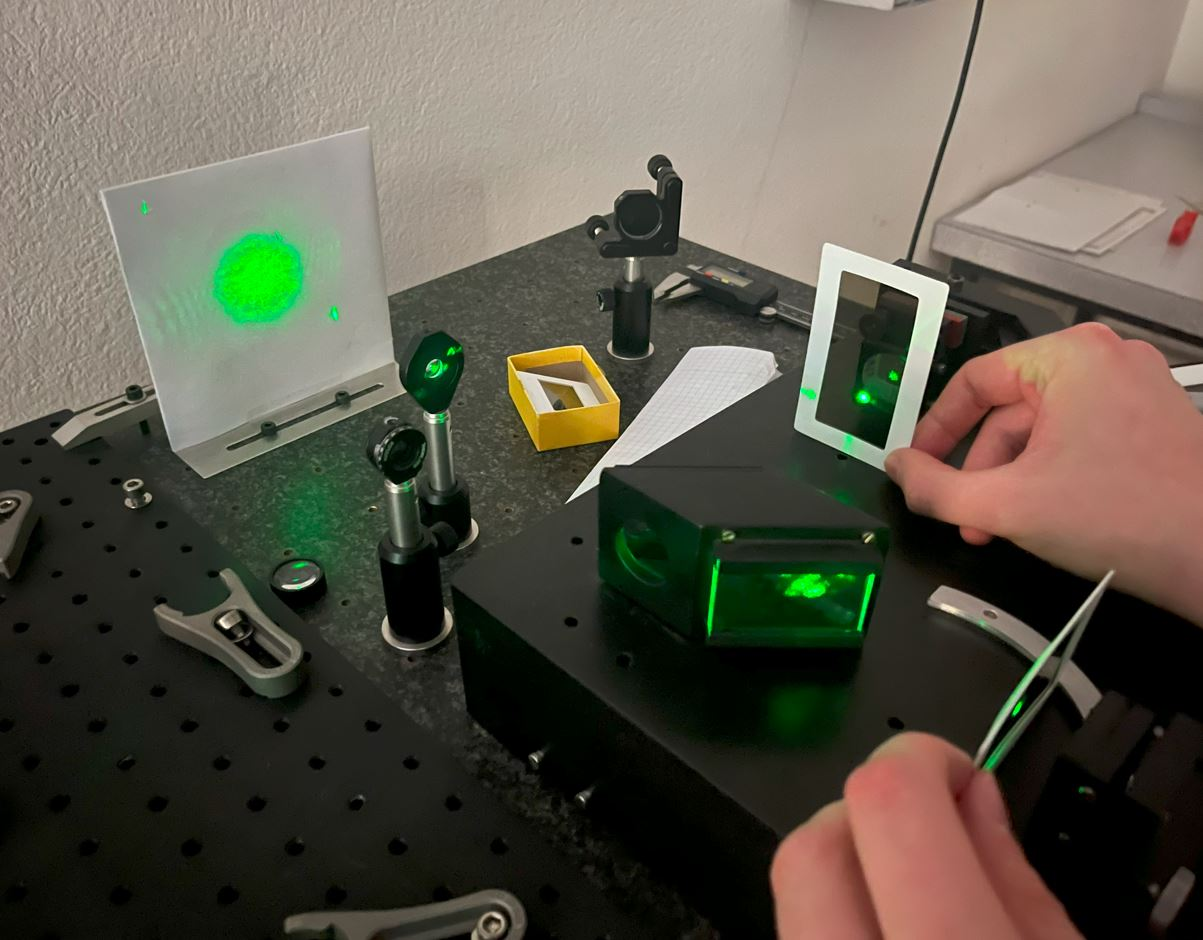
\includegraphics[width=\textwidth]{./figures/Interferometer_polarisation_normal.JPG}
		\caption{Normale Ausrichtung der Polarisationsfilter
		}\label{fig:interferometer_polarisation_normal}
	\end{subfigure}
	\caption[Sichtbares Interferenzmuster mit der Linse nach dem Beamsplitter und mit
		Verwendung von Polarisationsfiltern] {Sichtbares Interferenzmuster mit der
		Linse nach dem Beamsplitter und mit Verwendung von Polarisationsfiltern
	}\label{fig:interferometer_polarisation}
\end{figure}

Die Krümmung der Interferenzstreifen in
\autoref{fig:interferometer_polarisation_parallel} lässt sich dadurch erklären,
dass die Polarisationsfolien nicht perfekt gerade in den Lichtarm eingebracht
werden. Sind die Polarisationsfolien normal zueinander ausgerichtet, wie in
\autoref{fig:interferometer_polarisation_normal} ist kein Interferenzmuster
sichtbar, weil die beiden Lichtstrahlen aufgrund ihrer Ausrichtung nicht
miteinander Interferieren können.

\section{Auswertung}\label{sec:auswertung}

Um zu sehen wie sich die Unsicherheit der Messungen bis in die Ergebnisse
fortpflanzt, ist erweiterte Gauss-Methode verwendet worden. Die Grundlagen
dieser Methode stammen von den Powerpointfolien von
GUM~\cite{wolfgangkesselISOBIPMGUMSicht2004}. Für die Auswertung ist die
Progammiersprache Python im speziellen die Pakete \verb#labtool-ex2#,
\verb#pandas#, \verb#sympy#, \verb#lmfit# zur Hilfe genommen worden.
\verb#lmfit# wurde für das Fitten verwendet, \verb#sympy# wurde für symbolische
Manipulation verwendet und die restlichen Pakete für leichteres Handhaben der
Daten. Dies wurde aber alles durch \verb#labtool-ex2# abstrahiert.

Um höchstmögliche Genauigkeit zu garantieren wird erst bei der Darstellung der
Wert in Tabellen gerundet.

\subsection{Young'scher Doppelspalt, Beugungsgitter}\label{sec:ausw_doppelt}

% Berechnen Sie die Beugungsmuster für die Doppelspalten 1-4 (die Spaltbreiten
% und -abstände sind in der Tabelle angegeben) und vergleichen Sie mit dem
% Experiment. Stellen Sie dazu jeweils einzeln den Interferenzterm und den
% Beugungsterm dar, sowie das gesamte Beugungsmuster. Vergleichen und erklären
% Sie auf Basis der berechneten Muster insbesondere die Lage der 1. Nebenmaxima
% der Doppelspalte 1 und 2.
Um die Wellelängen des LASERs bestimmen zu können wurden die Distanz
$\Delta x$ zwischen den zwei Maximal auseinanderliegendene Intensitätmaxima und
die Anzahl der Maxima $N$ zwischen diesen minus dem Nullten bestimmt werden.
Dabei wurden nur die durch den Einzelspalt verursachten Maxima gezählt und
aus den Bilder herausgemessen. Da nun nach
\autoref{eq:konstruktiveInterferenz} für große Distanzen die Intensitätsmaxima
äquidistant von einander entfernt sind, muss die Distanz $\Delta x$ noch durch
die Anzahl der Maxima $N$ dividiert werden um den effektiven Abstand zwischen zwei Maxima zu
finden. Dann kann durch Umformen der \autoref{eq:konstruktiveInterferenz}
auf die Wellenlänge $\lambda$ geschlossen werden:

\begin{table}[H]
	\centering
	\caption{Diese Tabelle beinhaltet aus den Bildaufnahmen der Intensitätsverteilung 
  aufgenommen Werte unter Verwendung verschiedener Doppelspälte. Dabei gilt: \\
$\Delta x \dots$ Distanz zwischen den Zwei am weitesten entfernten ablesbare Maxima \\
$N \dots$ Anzahl der Maxima vom Linkesten bis zum Rechtesten, wobei nur 
die Maxima der Einzelnensplaltinteferenz gezählt werden\\
$d \dots$ Spaltabstand \\
$\lambda \dots$ Errechnete Wellenlänge 
}\label{tab:auswertungWellenlangenDoppelspalt}
	\begin{tblr}{row{1}={font=\mathversion{bold}},colspec={S[table-format=3.0(2)]S[table-format=2.1(1)]S[table-format=1.1(1)]S[table-format=1.1(1)e1]}}
{{{$\Delta x$ / \si{\mm}}}} & {{{$N$ / 1}}} & {{{$d$ / \si{\mm}}}} & {{{$\lambda$ / \si{\meter}}}}\\
162(10) & 12.0(0) & 0.1(0) & 5.4(4)e-07\\
149(10) & 12.0(0) & 0.1(0) & 4.9(4)e-07\\
161(10) & 12.0(0) & 0.1(0) & 5.3(4)e-07\\
152(10) & 24.0(0) & 0.2(0) & 5.1(4)e-07\\
\end{tblr}

\end{table}

Diese Wellenlängen ergeben gemittelt:

\begin{equation*}
	\lambda = \SI{518(17)}{\nm}
\end{equation*}

Nun werden die Interferenzmuster Bezüglich der Intensität mit den theoretischen Verläufen
verglichen. Dazu wird mittels den ersten Paar periodischen Dunkelpeaks der
Maßstab bestimmt, welcher für das ganze Interval extrapoliert werden kann.
Damit können den Pixelwerten nun Distanzen zugeordnet werden. Für diese
Distanzen werden nun auch die theoretischen Interferenzmusterverläufe aus
\autoref{eq:InterferenzDoppelSpalt}, \autoref{eq:InterferenzEinzelspalt} und
deren Superposition ausgewertet, was in
\autoref{fig:auswertung_intensity} sichtbar ist.

\begin{figure}[H]
	\centering
	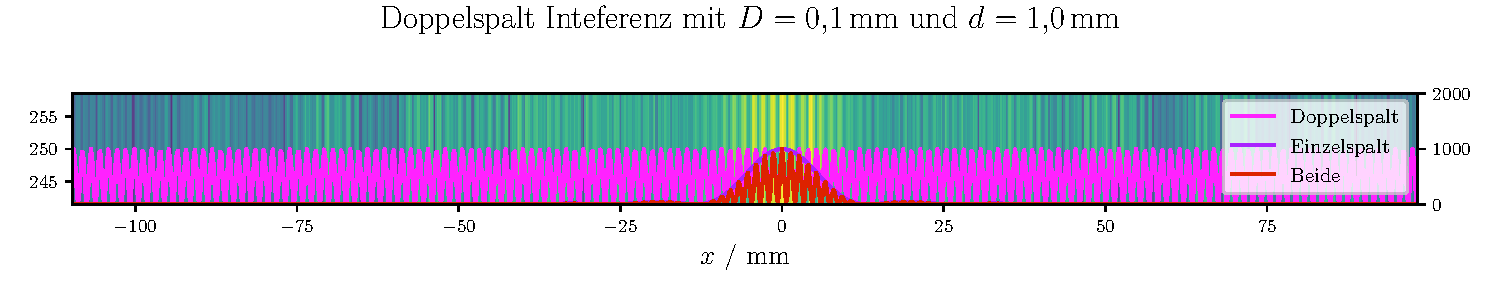
\includegraphics[width=0.95\textwidth]{figures/intensity_1.pdf}
	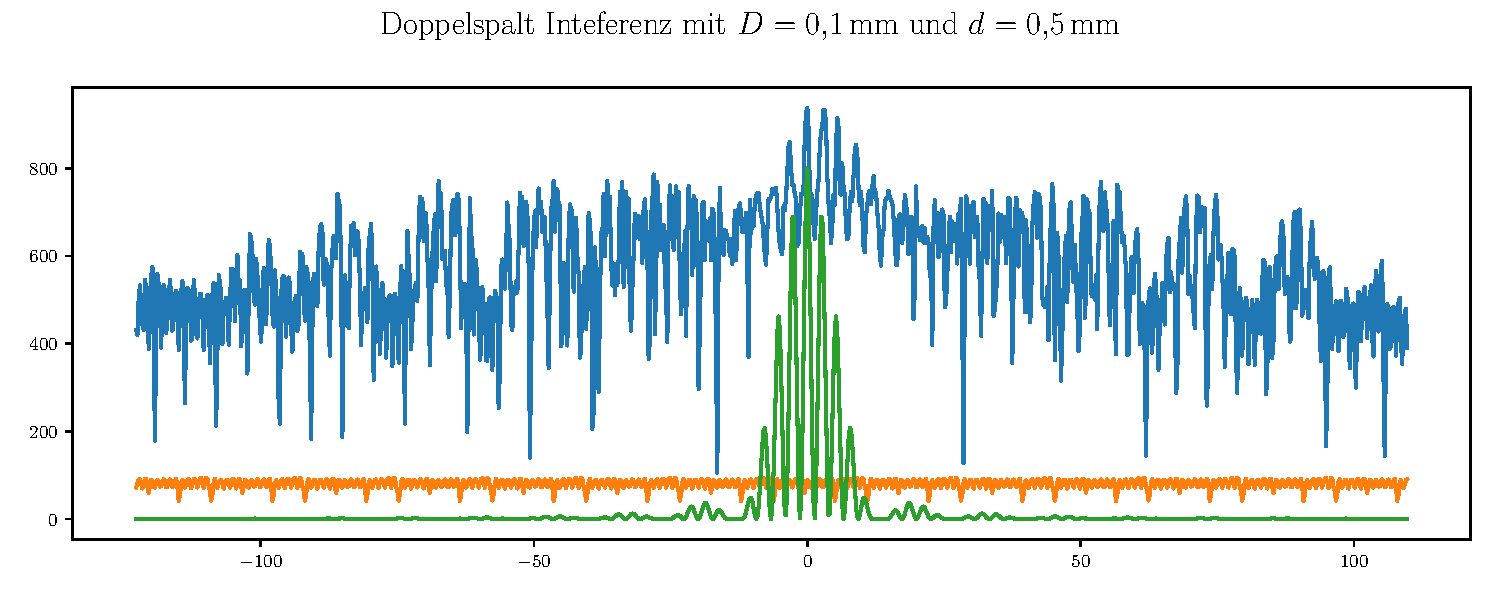
\includegraphics[width=0.95\textwidth]{figures/intensity_2.pdf}
	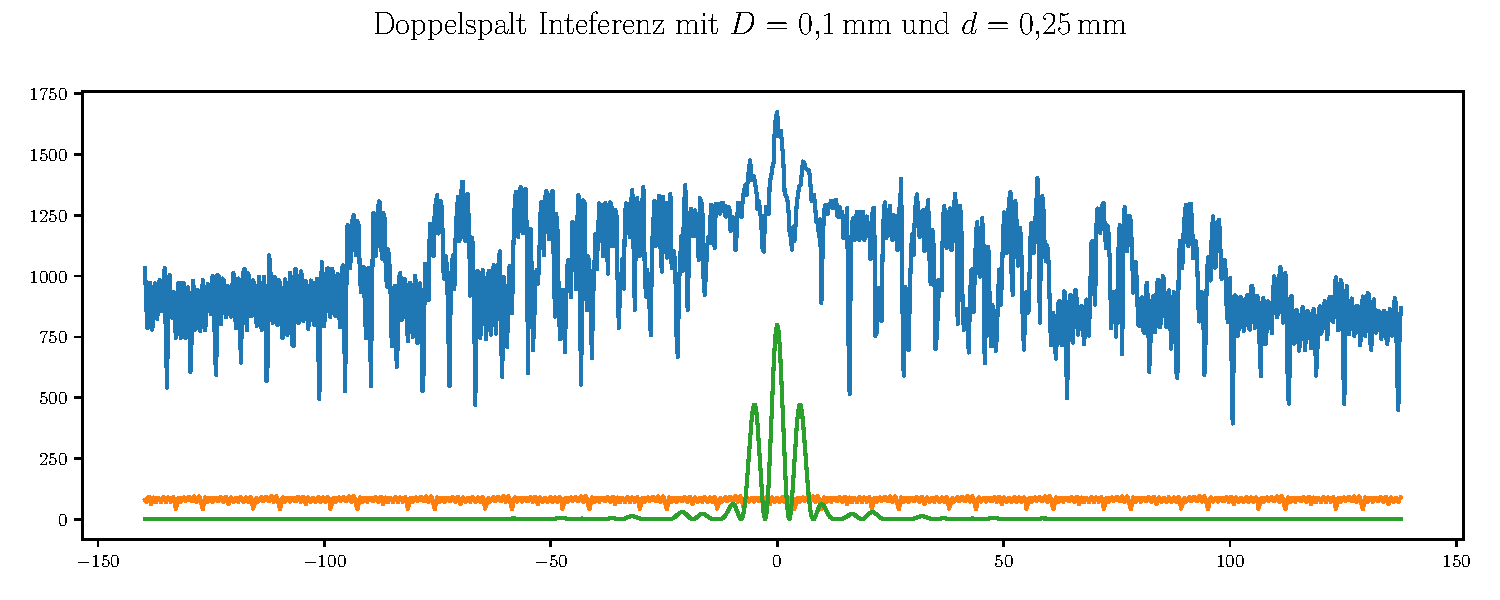
\includegraphics[width=0.95\textwidth]{figures/intensity_3.pdf}
	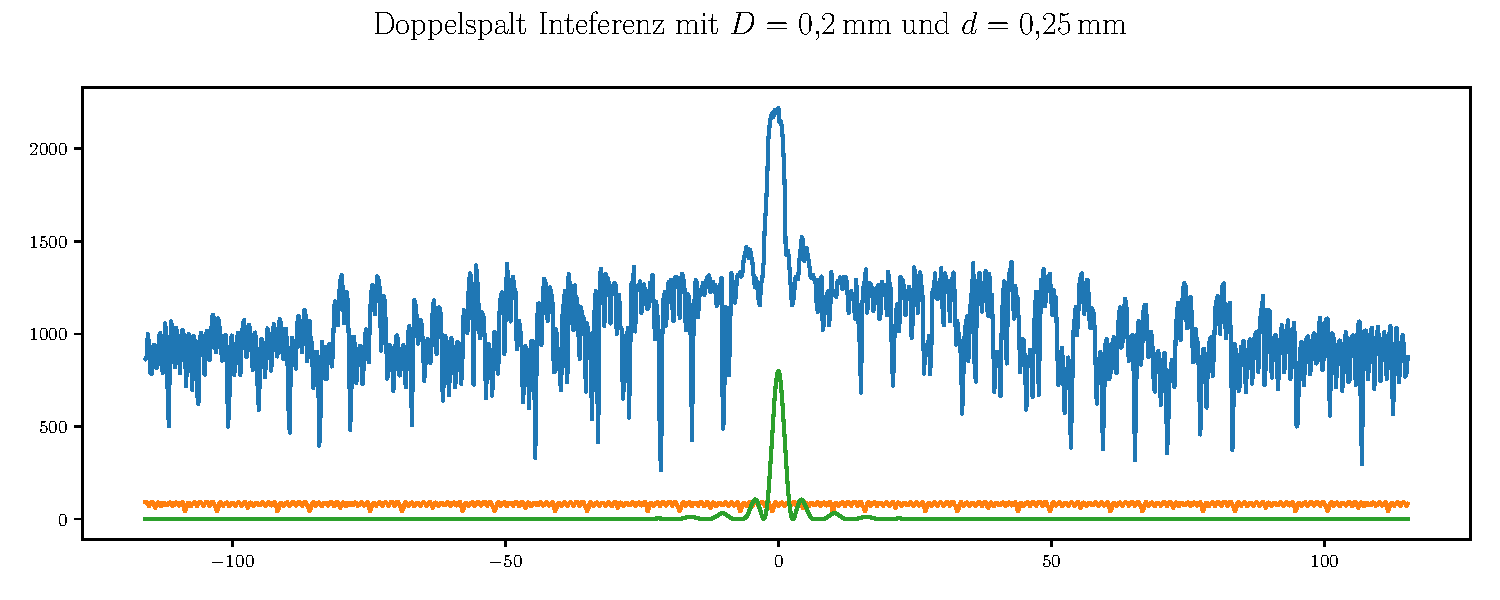
\includegraphics[width=0.95\textwidth]{figures/intensity_4.pdf}
	\caption{In dieser Graphik sind die theoretischen und
  gemessenen Verläufe der Intensitäten bei verschiedenen Doppelspälte 
  qualitativ dargestellt. Im Hintergrund sind die gemessenen 
  Helligkeitsdaten sichtbar, im Vordergrund die theoretischen Verläufe.
Dabei bezeichnet $D$ die Spaltdicke und 
$d$ den Spaltabstand zwischen den beiden Einzelspalten.}\label{fig:auswertung_intensity}
\end{figure}

% Vermessen oder fotografieren Sie das Beugungsmuster und bestimmen Sie die Gitterkonstante.
Analog zu der Beugung am Doppelspalt wurde die maximale Distanz zwischen zwei
Maxima auf dem Millimeterpapier genommen und die Anzahl der Maxima dazwischen gezählt. Mit
dieser Information und dem Gitterbeugungsgesetzt von Bragg lässt sich die
Gitterkonstante des Gitters bestimmen. Hier wurde die oben errechnete
Wellenlänge für den LASER verwendet, um die Gitterkonstante zu bestimmen. Die
Gitterkonstante $g$ ergibt sich folgendes:

\begin{enumerate}
	\item $N = \num{24}$
	\item $\Delta x = \SI{0.2720(10)}{\m}$
	\item $g = \SI{115(6)}{\um}$
\end{enumerate}

\subsection{Polarisation}

% Stellen Sie die winkelabhängige Transmission zusammen mit dem berechneten Verlauf graphische dar.
Die erhaltenen Werte aus \autoref{tab:werte_polarisation} werden nun in einem
Scatterplot dargestellt, dabei wurde als Vergleich der theoretische Verlauf des
Malus-Gesetzs als durchgängige Linie eingezeichnet. Für die eingehende Beleuchtungsstärke ist die
Hälfte der Beleuchtungsstärke ohne Polarisatoren genommen worden, welche zu
\SI{1200(200)}{\lux} gemessen wurde.

\begin{figure}[H]
	\begin{center}
		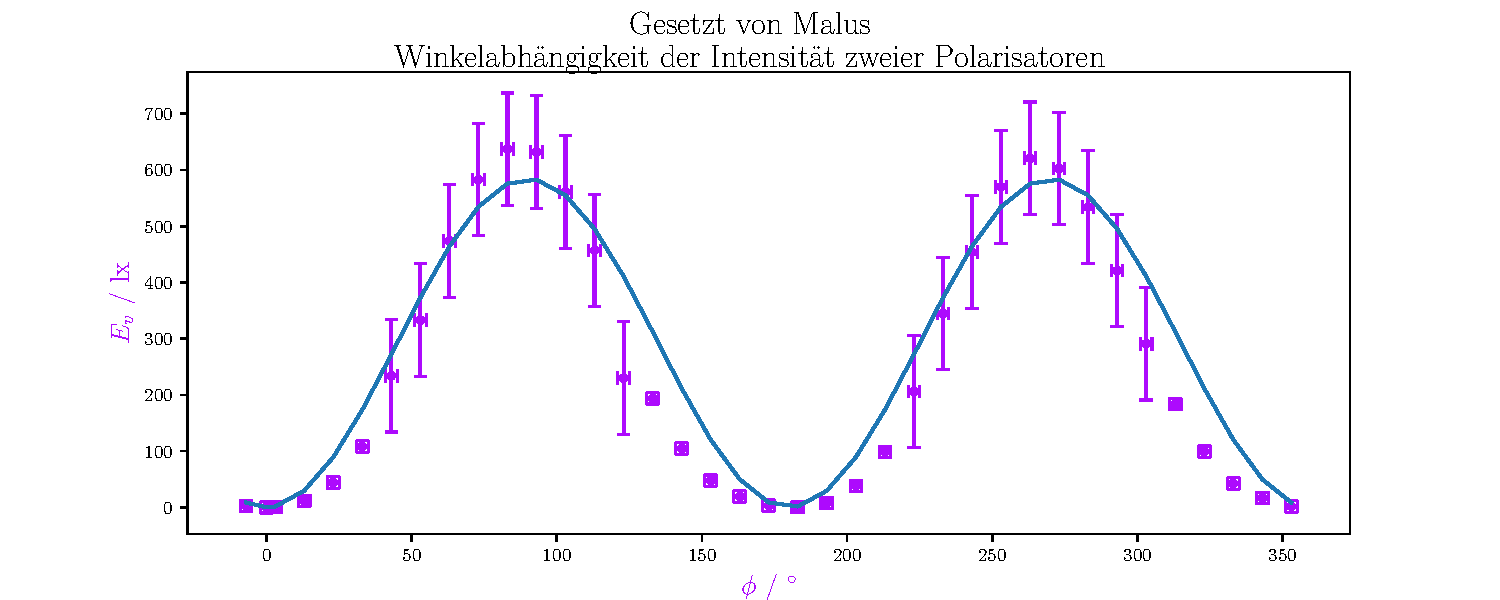
\includegraphics[width=0.95\textwidth]{figures/pol.pdf}
	\end{center}
	\caption{In dieser Graphik ist der theoretische Verlauf vom Malus-Gesetz
    dem vom Experiment erhaltenen gegenübergestellt worden. Dabei ist $E_v$ 
    die Beleuchtungsstärke am Sensor nach den Polarisatoren und $\phi$ der
    Winkel zwischen den Polarisatoren. Für den theoretischen Verlauf ist die 
    eingehende Beleuchtung als $E_{v_0}=\SI{600(100)}{\lux}$ (durch eine Messung bestimmt)
    angenommen worden.
  }\label{fig:auswertung_polarisation}
\end{figure}

% KEINE AUSWERTUNG NOETIG Bringen Sie nun zwischen zwei gekreuzte Polarisatoren einen weiteren
% Polarisator ein (Polarisationsfolie). Beobachten Sie die jeweilige Transmission
% durch das Gesamtsystem und erklären Sie die Beobachtungen mit dem Gesetz von
% Malus.

\subsection{Michelson Interferometer}

% Bestimmen Sie durch Verfahren des Spiegels SP2 die Wellenlänge des LASERs. Zählen Sie dazu die beim Verfahren der Mikrometerschraube 
% um x im Zentrum des konzentrischen Intensitätsmusters auftretende Anzahl N der
% Maxima (oder Minima). Achtung: Die Längenänderung der den Spiegel bewegenden
% Mikrometerschraube wird durch einen Hebel um den Faktor 5,3 untersetzt, die
% tatsächliche Spiegelbewegung ist also x‘=x/5,3. Somit gilt  = 2x‘/N.
% Bestimmen Sie selbst die Anzahl der registrierten Übergänge um den Fehler
% möglichst zu minimieren.

Zunächst wurden für die Distanzen $s$ und deren Ordnungszahl $N$ die Differenzen 
zwischen den Einträgen und ihren nächsten Nachbarn gebildet. Durch
Division von $\Delta s$ durch $\Delta N$ und dem Mitteln der Resultate lässt sich
die Wellelänge $\lambda$ gleich wie in \autoref{sec:ausw_doppelt} mittels
\autoref{eq:konstruktiveInterferenz} bestimmen.

Somit ergibt sich für die Wellenlänge:
\begin{equation*}
	\lambda = \SI{580(30)}{\nm}
\end{equation*}

\section{Diskussion}\label{sec:diskussion}


\subsection{Young'scher Doppelspalt, Beugungsgitter}

Um die Distanzmessung zwischen den Beugungsmaxima möglichst genau durchführen
zu können, wurde Millimeterpapier am Schirm verwendet. Bezüglich der Auswertung
der Fotos sei angemerkt, dass sich durch die Abbildung mithilfe der Kamera eine
gewisse Verzerrung des Bildes nicht vermeiden lässt, was sich auf die erzielte
Unsicherheit auswirkt und durch ein entsprechendes Sensorsystem verbessert
werden könnte. Diese Verzerrung verursacht auch die Diskrepanz zwischen den
theoretischen Verlauf und dem Gemessen, dies verursacht nun eine Verschiebung
der Frequenz und der Offsets.

Ein Verbesserungsvorschlag für eine automatische Auswertung wäre die Verwendung eines Photodetektorarrays. 
Dadurch würde automatisch der Maßstab der Distanzen zu den Pixeln ohne Verzehrung dargestellt werden. Ist dies jedoch
nicht möglich wird Empfohlen die Intesitätsverteilung nicht am Millimeterpapier sonder über dem 
Grid am weißen Bereich auszulesen. Dadurch beeinflusst die schwarze Farbe der Millimeterskalen
die Absportionscharakteristik nicht, welche hier jedoch in den Daten zu sehen waren und zum
Erstellen des ``Pixel-Distanz'' Maßstabs verwendet wurden.

\subsection{Polarisation}

Die beiden Polarisationsfilter werden auch außerhalb des Versuchsaufbaus vor
eine Lichtquelle gehalten und zueinander verdreht. Dadurch wird festgestellt,
dass die 0-Position an beiden Polaristatoren beinahe dazu führt, dass kein
Licht durchgelangt. Dies deckt sich auch mit dem erzeugten Intensitätsverlauf
in \autoref{fig:auswertung_polarisation}.

Generell decken sich die erhaltenen Ergebnisse mit dem Gesetz von Malus. Auch
die Ergebnisse bei der Verwendung von 3 Polarisationsfolien entsprechen jenen,
die durch die Theorie vorausgesagt wurden. Nämlich, dass durch das Hinzufügen
eines Dritten Polarisators die Intesität, bei einer Verdrehung der zwei
anderen Polarisatoren von \SI{90}{\degree}, ungleich null ist, wenn dieser
nicht in eine der zwei Polarisationebenen gedreht ist.

Um eine ideale Messung zu garantieren wäre es angebracht, den gesamten Raum
abzudunkeln, um eventuelles Hintergrundlicht bestmöglich zu reduzieren. Da im
gleichen Raum ein weiterer Versuch von einer Anderen Gruppe durchgeführt wurde,
konnte dies nicht vollständig realisiert werden.

Die Abweichungen können durch die elliptischen Eigenschaft der Laserquelle beschrieben werden.
Durch 

% TODO Bild

Ein Verbesserungsvorschlag wäre, noch eine Übersetzung für den Winkel hinzuzufügen.
Hier würde sich im Speziellen ein Schneckengetriebe anbieten, wo auch ein Durchlauf Servomotor
montiert werden kann um den genauen Winkel ansteuern zu können.
Weiters kann eine unpolarisierte Lichtquelle verwendet werden, damit keine Fehler beim
Verdrehen entstehen können und die Voraussetzungen des Malus-Gesetzes gegeben sind.


\subsection{Michelson Interferometer}

Aufgrund der Geometrie des Aufbaus, entspricht ein Durchlauf eines
Interferenzbildes der halben Wellenlänge des LASERs, wie bereits in
\autoref{sec:Grund} erklärt. Dies deckt sich auch mit dem beobachten
Resultaten, die erhaltene Wellenlänge stimmt mit dem LASER überein.

Die Beobachteten Effekte bezüglich Polarisation und Sensitivität auf
Erschütterungen decken sich mit der erwarteten Theorie. Insgesammt sei daher
nochmals erwähnt, dass das Interferometer sehr sensitiv auf eventuelle
Erschütterungen reagiert, was einen nicht zu vernachlässigenden Einfluss auf
die Messergebnisse hat. Ein Verbesserungsvorschlag hierzu wäre, den Versuch im
Keller des Gebäudes durchzuführen und nicht im Dachgeschoss.

\newpage

\section{Zusammenfassung}\label{sec:zusammenfassung}

Hier werden nochmals alle Ergebnisse dieser Experimentenfolge aufgelistet.
Wobei die meisten zu erstellenden Diagramme Aufgrund der Länge der
\autoref{sec:auswertung} entnommen werden sollen.

\subsection{Young'scher Doppelspalt, Beugungsgitter}

Hier werden die durch den Doppelspalt ermittelte Wellelänge des LASERs
$\lambda$ und die Gitterkonstante $g$ des Gitters angeführt.

\begin{enumerate}
	\item $\lambda = \SI{518(17)}{\nm}$
	\item $g = \SI{115(6)}{\um}$
\end{enumerate}

\subsection{Polarisation}

Für die Verifizierung des MalusGesetzt sei auf den erzeugten Verlauf in 
\autoref{fig:auswertung_polarisation} hingewiesen.

\subsection{Michelson Interferometer}
Hier wird die durch das Michelson-Interferometer ermittelte Wellelänge des LASERs
$\lambda$ angeführt.
\begin{enumerate}
	\item $\lambda = \SI{580(30)}{\nm}$
\end{enumerate}

\newpage
\printbibliography
%todo literatur
\listoffigures
\listoftables
\end{document}
